\documentclass[11pt,letterpaper]{article}
\usepackage[utf8]{inputenc}
\usepackage[T1]{fontenc}
\usepackage[spanish,es-tabla]{babel}
\usepackage{lmodern}
\usepackage{amsmath,amssymb,amsthm,mathtools}
\usepackage[margin=1.05in]{geometry}
\usepackage{graphicx}
\usepackage{booktabs}
\usepackage{array}
\usepackage{hyperref}

\newtheorem{theorem}{Teorema}
\newtheorem{lemma}{Lema}
\newtheorem{proposition}{Proposición}

\title{\textbf{Barreras de Bellman Afines Dependientes del Estado, Equivalencia Asintótica y la Curva en U Institucional}\\[0.5em]
\large Extensiones Analíticas, Certificados Reforzados y Microfundaciones sobre \emph{Minimum Viable Scale} (Milei y Reidel, 2026)}
\author{Marcelo Segura\thanks{Documento Técnico de Trabajo (preprint). El desarrollo analítico, la edición técnica y las rutinas de verificación simbólica y numérica en Python contaron con asistencia de herramientas de inteligencia artificial bajo la dirección, supervisión crítica y plena responsabilidad del autor.}}
\date{Noviembre 2026}

\begin{document}
\maketitle

\begin{abstract}
Este trabajo desarrolla cuatro contribuciones analíticas y extensiones estructurales sobre el modelo de supervivencia óptima con rendimientos crecientes a escala, complementariedad bruta y trabajo endógeno de Milei y Reidel (2026, \emph{Minimum Viable Scale: Bellman Barriers and the Economics of Survival}). \textbf{Primero}, en el certificado de Barreras de Bellman de Primer Paso (FPBB) de la Sección 7.2, identificamos un término de holgura omitido en la construcción en bloques de dos períodos: al comparar cualquier transición individual $(x,y)\in M\times M$ con el par $(h,b)$ a igual esfuerzo laboral, la ganancia de consumo retiene simultáneamente el diferencial de capital inicial $q(h-x)$ y el diferencial de ahorro $(y-b)$. Mediante una barrera afín dependiente del estado $B_1(x)$ de un solo paso, reducimos el techo de la barrera en casi cinco unidades ($-43.0465$ frente a $-38.1442$), \textbf{casi triplicamos el margen de calibración de permanencia} (de $2.564$ a $7.4665$ uniforme y $7.7756$ en $b=0.10$) y \textbf{reducimos a la mitad el plazo máximo certificado de entrada} a $H=[0.28,\infty)$ (de $46$ a \textbf{$23$ períodos}, $24$ uniforme). Extendemos además el certificado a la banda previa $M_0=[0.05,0.10)$ con cota explícita $\tau_{.1}\le 10$ períodos, y certificamos analíticamente mediante descomposición de Wronskiano y aritmética de intervalos que la Tabla 5 de salidas adversas ($12$ subintervalos finitos) colapsa a dos evaluaciones en frontera sin mínimos interiores, elevando el margen de salida en $M$ de $0.0436$ a $>0.0947$ y el margen global FPBB de $0.0423$ ($0.04$) a \textbf{$>0.0571$} ($+35\%$). \textbf{Segundo}, resolvemos la pregunta abierta de la Nota al pie 1 estableciendo el isomorfismo finito $S_A^{\mathrm{fix}}(\overline{L}) = \overline{L}\,S_{A\overline{L}^r}^{\mathrm{fix}}(1)$, formulando una condición variacional precisa para $S_A^{\mathrm{fix}}(1) < S_A$, y demostrando bajo la condición de paciencia que cuando $A\to\infty$ tanto la frontera con trabajo endógeno como con trabajo fijo convergen a $s_\infty^*=(\delta/c_K)^{1/r}$ ($S_A/S_A^{\mathrm{fix}}(\overline{L})\to 1$), respaldado numéricamente por iteración de función de valor (VFI). \textbf{Tercero}, microfundamos la Sección 4.3 mediante gasto público productivo tipo Barro (1990) y carga regulatoria improductiva $(\tau_p,\tau_u)$, separando la curva en U exacta de la cota certificada $\overline{S}(\tau)$ y del piso físico $\kappa(\tau)$, la simetría por pares de $S(\tau)$ a $A_0$ finito y el perfil límite asintótico cuando $A_0\to\infty$. \textbf{Cuarto}, formalizamos la descentralización empresarial manteniendo la contabilidad factorial exacta $(\theta/\mu)Y_t$, el crecimiento sin techo en unidades de eficiencia y los certificados estocásticos de Bellman bajo un proceso Markoviano explícito mediante parada opcional de Doob.

\medskip
\noindent\textbf{Palabras clave.} escala mínima viable; barreras de Bellman de primer paso (FPBB); cotas de tiempo de entrada; oferta laboral endógena; curva en U institucional.\\
\noindent\textbf{Códigos JEL.} C61, D24, D61, H21, O41.
\end{abstract}

\section{Introducción}

En \emph{Minimum Viable Scale: Bellman Barriers and the Economics of Survival}, Milei y Reidel (2026) establecen una teoría unificada de la supervivencia económica cuando la tecnología agregada exhibe rendimientos crecientes a escala ($1<\theta<2$), complementariedad bruta entre capital y trabajo ($\rho=-d<0$) y oferta laboral endógena con utilidad logarítmica sobre el consumo y el ocio ($L\in[0,1]$). Su resultado central muestra que, bajo una condición de paciencia ($\beta[q+\theta\delta]>1$) y productividad suficientemente elevada ($A>A_*$), existe una única Escala Mínima Viable $S_p$ estrictamente superior al umbral de reposición física $\kappa_p$ (\textbf{Teorema 1}). En la banda intermedia $(\kappa_p,S_p)$, aunque es físicamente factible sostener el stock de capital indefinidamente con consumo y ocio positivos, todo sendero óptimo decide liquidar gradualmente el capital hacia la extinción porque el retorno neto futuro no compensa el sacrificio de consumo y ocio presentes. En la frontera $S_p$, las trayectorias óptimas de extinción y supervivencia coexisten alcanzando el mismo bienestar total pero generando un quiebre hacia arriba (\emph{upward kink}) en la función de valor (\textbf{Teorema 2}). Adicionalmente, dado que las sendas de liquidación diferida aproximan arbitrariamente bien el bienestar inicial óptimo (\textbf{Proposición 3}), los autores introducen el método de \textbf{Barreras de Bellman de Primer Paso} (\emph{First Passage Bellman Barriers}, FPBB) para certificar analíticamente el ingreso en tiempo finito a una región productiva objetivo $H$ sin resolver la función de valor exacta $V_p(K)$.

Pese al rigor del marco de Milei y Reidel (2026), un análisis detenido de su construcción computacionalmente verificada en la Sección 7 y el Apéndice F, así como de las preguntas abiertas señaladas en el cuerpo del artículo, revela cuatro brechas analíticas susceptibles de cierre preciso sin alterar los axiomas del modelo ni ampliar su caja paramétrica:

\begin{enumerate}
\item \textbf{Afilamiento simultáneo de la barrera de permanencia y certificación global de las salidas adversas (Sección 3):} En el Teorema 9 de Milei y Reidel (2026), sobre la caja paramétrica (7.3) para la región de tránsito $M=[0.10,0.28)$ y la región objetivo $H=[0.28,\infty)$, una barrera constante es imposible porque en el extremo superior $h=0.28$ la recompensa de liquidar hacia $b=0.10$ supera el bienestar alcanzable desde $b$. Los autores sortean esta obstrucción construyendo una barrera de bloques de $N=2$ períodos que arroja $B(K)\le -38.144176$, un margen de permanencia $>2.564$, un plazo máximo de entrada de $\tau_H\le 46$ períodos y un margen global del certificado de $0.04$ (cuyo mínimo en su Tabla 5 es $0.0423$). Demostramos en el \textbf{Lema 1} y el \textbf{Teorema 9*} que el agrupamiento en pares de la ecuación (7.6) descarta aproximadamente la mitad de la disipación disponible en cada transición individual $(x,y)\in M\times M$: una barrera afín de \emph{un solo paso} $B_1(x)$ retiene ambos términos simultáneamente, mejora la cota superior de la barrera a $-43.046512$, eleva el margen de permanencia a \textbf{$>7.4665$} ($>7.7755$ en $b=0.10$) y reduce exactamente a la mitad el plazo máximo de entrada a \textbf{$\tau_H\le 23$ períodos} ($24$ uniforme). Asimismo, cerramos la brecha sin cota de la Figura 6 en la banda previa $M_0=[0.05,0.10)$ certificando \textbf{$\tau_{.1}\le 10$ períodos} (\textbf{Proposición 1*}) y demostramos mediante un certificado de aritmética de intervalos sobre el Wronskiano y la segunda derivada (\textbf{Proposición 1**}) la ausencia de mínimos interiores en $M$ y $H_1$, reduciendo la Tabla 5 original a dos evaluaciones en frontera que elevan el margen de salida en $M$ a $>0.0947$ y el margen global FPBB a \textbf{$>0.0571$} ($+35\%$).

\item \textbf{Resolución asintótica e isomorfismo finito entre trabajo endógeno y fijo (Sección 4):} En la Nota al pie 1 (página 2), Milei y Reidel (2026) dejan como pregunta abierta la comparación entre la frontera $S_A$ con trabajo endógeno y la frontera $S_A^{\mathrm{fix}}(\overline{L})$ con trabajo exógenamente fijo. En el \textbf{Teorema 3*} probamos el isomorfismo exacto para todo $A$ finito, $S_A^{\mathrm{fix}}(\overline{L}) = \overline{L}\,S_{A\overline{L}^r}^{\mathrm{fix}}(1)$, formulamos la condición variacional exacta bajo la cual $S_A^{\mathrm{fix}}(1) < S_A$, y demostramos que bajo la condición de paciencia (2.3) (la cual fuerza $\beta\theta>1$) tanto $A^{1/r}S_A$ como $A^{1/r}S_A^{\mathrm{fix}}(\overline{L})$ convergen al límite físico común $(\delta/c_K)^{1/r}$, cerrando el cociente $S_A/S_A^{\mathrm{fix}}(\overline{L})\to 1$ cuando $A\to\infty$, junto con una verificación numérica directa de fronteras por VFI.

\item \textbf{Microfundación institucional y curva en U fiscal--regulatoria (Sección 5):} En la Sección 4.3, los autores modelan distorsiones mediante una pérdida multiplicativa exógena $A_e=(1-\tau)A$, advirtiendo expresamente que su aplicación a impuestos o regulaciones exige contabilizar los beneficios productivos de los ingresos recaudados. Acoplando la tecnología CES con provisión pública equilibrada de infraestructura y derechos de propiedad tipo Barro (1990) junto con carga burocrática improductiva ($\tau=\tau_p+\tau_u$), derivamos el \textbf{Teorema 10}: caracterizamos las dos trampas físicas de extinción ($\tau<\tau_{\min}$ y $\tau>\tau_{\max}$), establecemos la curva en U diferenciable exacta tanto para el piso físico $\kappa(\tau)$ como para la cota superior certificada $\overline{S}(\tau)$ con mínimo único en $\tau^*=\alpha/(1+\alpha)$, probamos la simetría de conjuntos de nivel de $S(\tau)$ para todo $A_0$ finito y su perfil límite exacto cuando $A_0\to\infty$, además de la monotonicidad estricta frente a burocracia improductiva $\tau_u$.

\item \textbf{Descentralización empresarial, crecimiento sostenido y barreras estocásticas (Sección 6):} Finalmente, extendemos el núcleo determinista de planificador central con techo estacionario $K_p^+$ en tres direcciones: (i) descentralización bajo competencia monopolística (Dixit y Stiglitz, 1977) con contabilidad factorial exacta $(\theta/\mu)Y_t$ y externalidades (Romer, 1986), probando que fragmentar empresas en $M$ unidades equivale a destruir productividad según $A/M^{\theta-1}$ (\textbf{Proposición 2*}); (ii) crecimiento balanceado aumentador de trabajo a tasa $g>0$, que elimina el techo $K_p^+$ y genera despegue exponencial perpetuo («palo de hockey») preservando cada certificado en unidades de eficiencia (\textbf{Proposición 3*}); y (iii) extensión probabilística de las FPBB bajo condiciones explícitas de integrabilidad y transiciones Markovianas de régimen mediante el Teorema de Parada Opcional de Doob (\textbf{Teorema 11}), cuantificando cómo reducir $\tau_H$ de $46$ a $23$ eleva al cuadrado la cota de supervivencia $(1-p)^{\tau_H}$ ante shocks severos.
\end{enumerate}

El resto del artículo se organiza como sigue. La Sección 2 sitúa nuestras contribuciones en la literatura económica y de control óptimo verificado. La Sección 3 desarrolla las barreras afines de un paso, la cota de cruce previo y la reducción de la Tabla 5. La Sección 4 resuelve la Nota al pie 1 y presenta la verificación numérica asintótica. La Sección 5 deriva la curva en U institucional y descompone gasto productivo frente a peso muerto regulatorio. La Sección 6 formaliza la descentralización, el crecimiento sin techo y las barreras estocásticas. La Sección 7 concluye.

\section{Literatura Relacionada y Posicionamiento Teórico}

Nuestros resultados se articulan en la intersección de cuatro líneas de investigación económica y matemática, cerrando en cada una limitaciones específicas respecto de las pruebas cuantitativas de supervivencia y las implicancias institucionales del modelo de Milei y Reidel (2026).

\subsection{Crecimiento óptimo no cóncavo, umbrales de Skiba y trampas de pobreza}

Desde las contribuciones pioneras de Skiba (1978), Majumdar y Mitra (1982) y Dechert y Nishimura (1983), la teoría del crecimiento óptimo ha documentado que las tecnologías no convexas o con rendimientos crecientes locales dividen el espacio de estados mediante un umbral crítico de indiferencia donde coexisten trayectorias óptimas convergentes hacia la extinción o hacia un régimen próspero. Posteriormente, Mitra y Ray (1984) generalizaron las condiciones de existencia y monotonicidad a conjuntos factibles no convexos, mientras que Kamihigashi y Roy (2007) y Akao, Kamihigashi y Nishimura (2011) establecieron caracterizaciones globales en tiempo discreto sin diferenciabilidad ni concavidad, extendidas recientemente al tiempo continuo por Akao, Ishii, Kamihigashi y Nishimura (2022). En paralelo, la literatura de desarrollo económico formalizó trampas de pobreza basadas en externalidades de umbral en capital humano (Azariadis y Drazen, 1990) e imperfecciones crediticias con inversiones indivisibles (Galor y Zeira, 1993), mientras que Wagener (2020) caracterizó geométricamente los puntos de inflexión (\emph{tipping points}) mediante variedades de indiferencia y principios de envolvente. No obstante, como señalan Kraay y McKenzie (2014) al evaluar la evidencia empírica, la mayoría de los modelos teóricos clásicos de umbrales operan con trabajo fijo y solo demuestran convergencia asintótica cualitativa, sin acotar cuánto tiempo tarda una economía que supera el umbral crítico en alcanzar un régimen productivo autosostenido. Nuestro \textbf{Teorema 9*} y la \textbf{Proposición 1*} suplen precisamente esta carencia en el modelo con trabajo endógeno de Milei y Reidel (2026), proporcionando plazos explícitos de entrada garantizada ($\tau_{.1}\le 10$ y $\tau_H\le 23$ períodos).

\subsection{Oferta laboral endógena y complementariedad factorial bajo rendimientos crecientes}

La función de producción de elasticidad de sustitución constante (CES) introducida por Arrow, Chenery, Minhas y Solow (1961) desempeña un papel central cuando la elasticidad de sustitución entre capital y trabajo es inferior a la unidad ($\rho<0$), escenario documentado empíricamente por Klump, McAdam y Willman (2007) para economías agregadas. Cuando la tecnología CES se combina con elección endógena de horas trabajadas y utilidad no separable o dependiente del ocio, de Hek (1998) demostró que las preferencias consumo--ocio pueden engendrar multiplicidad de estados estacionarios y trampas de desarrollo incluso bajo tecnologías convexas, mientras que Benhabib y Farmer (1994) exhibieron indeterminación y fluctuaciones endógenas bajo rendimientos crecientes agregados. En el caso de Milei y Reidel (2026), la combinación de rendimientos crecientes ($1<\theta<2$), complementariedad bruta ($\rho=-d<0$) y desutilidad logarítmica del trabajo impide comparar directamente la frontera $S_A$ frente al modelo canónico de trabajo fijo (Nota al pie 1). Nuestro \textbf{Teorema 3*} resuelve esa comparación analítica: establece un isomorfismo exacto para productividad finita $A$ y prueba que, en el límite $A\to\infty$ sobre la escala crítica $A^{-1/r}$, el trabajo óptimo tiende a cero pero más lentamente que el capital ($K_t/L_t\to 0$), haciendo que el término de ocio desaparezca algebraicamente y ambos regímenes converjan al mismo problema límite.

\subsection{Barreras de Bellman, dualidad y certificados estocásticos de primer paso}

El método FPBB de Milei y Reidel (2026) conecta la programación dinámica clásica (Bellman, 1957; Stokey, Lucas y Prescott, 1989) y los teoremas de envolvente sin diferenciabilidad (Milgrom y Segal, 2002) con cuatro tradiciones técnicas: la viabilidad en horizonte finito (Bertsekas, 1972), las funciones de almacenamiento disipativo (Willems, 1972; Grüne, Müller, Kellett y Weller, 2021), los iterados finitos de Lyapunov en control no lineal (Geiselhart, Gielen, Lazar y Wirth, 2014; Noroozi, Geiselhart, Grüne y Wirth, 2020) y la dualidad de programación lineal y valoración de opciones americanas (Haugh y Kogan, 2004; Gaitsgory, Parkinson y Shvartsman, 2019). Sin embargo, la construcción aplicada de la Sección 7.2 de Milei y Reidel (2026) utiliza bloques de dos pasos ($N=2$) con una función de referencia constante, descartando la mitad de las ganancias de consumo por arista, y discretiza la región $M\cup H$ en doce intervalos finitos en su Tabla 5 para acotar salidas adversas. Al sustituir la referencia constante por una barrera afín dependiente del estado en un solo paso ($N=1$) y probar monotonía estricta de las holguras de salida adversa (\textbf{Proposición 1**}), reducimos a la mitad la cota de tiempo de entrada y elevamos el margen global certificado en un $35\%$. Más aún, mientras el FPBB original es estrictamente determinista, nuestro \textbf{Teorema 11} extiende el método al ámbito estocástico mediante supermartingalas y el Teorema de Parada Opcional de Doob (1953), conectando el plazo de entrada determinista con la probabilidad de sobrevivir shocks agregados en tránsito.

\subsection{Bienes públicos productivos, distorsiones regulatorias y estructura de mercado}

Finalmente, la Sección 4.3 de Milei y Reidel (2026) se apoya en la literatura moderna de mala asignación factorial y costos regulatorios ---donde Restuccia y Rogerson (2008), Hsieh y Klenow (2009), Garicano, Lelarge y Van Reenen (2016) y Trebbi, Zhang y Simkovic (2026) cuantifican cómo cuñas regulatorias dependientes del tamaño empresarial y cargas de cumplimiento deprimen la productividad total de los factores (TFP). Como advierten los propios autores (pág. 10), modelar impuestos o regulaciones únicamente como una pérdida pura $A_e=(1-\tau)A$ ignora el retorno productivo del gasto público y la protección de derechos de propiedad (Barro, 1990; Futagami, Morita y Shibata, 1993; Acemoglu, Johnson y Robinson, 2005). Nuestro \textbf{Teorema 10} unifica ambas perspectivas en una fórmula cerrada bivariada $A_e(\tau_p,\tau_u)=A_0\tau_p^\alpha(1-\tau_p-\tau_u)$ que reproduce la monotonía anti-burocracia de Milei y Reidel sobre $\tau_u$ y genera la curva en U sobre $\tau_p$. Asimismo, las extensiones de la Sección 6 muestran cómo descentralizar rendimientos crecientes sin pérdidas operativas mediante competencia monopolística (Dixit y Stiglitz, 1977) o externalidades de escala (Romer, 1986), revelando que fragmentar empresas en $M$ unidades replica exactamente un colapso de TFP $A/M^{\theta-1}$.

\section{Barreras de Bellman Afines de Un Paso, Plazo de Entrada y Afilamiento del Certificado Global}

\subsection{El marco paramétrico y la holgura en la construcción de dos períodos}

Siguiendo la Sección 7 de Milei y Reidel (2026), consideramos la tecnología CES armónica con parámetros $(\theta,\rho,w)=(3/2,-1,1/2)$, donde la función de producción y la utilidad por período son:
\begin{equation}
F_A(K,L) = A\left(\frac{2KL}{K+L}\right)^{3/2}, \qquad u(C,L) = \eta\log C + (1-\eta)\log(1-L), \qquad C + K' \le qK + F_A(K,L),
\end{equation}
sobre la caja paramétrica (7.3) del artículo original:
\begin{equation}
A\in[0.749,0.751], \qquad \beta\in[0.9699,0.9701], \qquad q\in[0.9199,0.9201], \qquad \eta\in[0.6999,0.7001].
\end{equation}
Para la región de tránsito $M=[b,h)=[0.10,0.28)$ y la región objetivo $H=[h,\infty)=[0.28,\infty)$, sea $r(K,s)=\max_{0\le L<1}\{\eta\log(qK+F_A(K,L)-s)+(1-\eta)\log(1-L)\}$ el retorno reducido en un período. Las constantes verificadas racionalmente en las ecuaciones (7.5) y la página 59 de Milei y Reidel (2026) son:
\[
\widehat{R} = -0.996 > r(h,b), \qquad \Delta_2 = 0.2997 < \frac{\eta_-\beta_-q_-(h-b)}{q_+ h + F_{A_+}(h,1)-b} = 0.2997787,
\]
con consumo máximo factible $C_{\max}=qh+F_A(h,1)-b \le C_{\max}^+ = 0.37495167$, piso del testigo en $M$ dado por $W_M(K)\ge W_M(b) > -35.579855 > -35.58$ y techo de continuación irrestricto $\Psi^\sharp(K)=\Psi(K)-10/301\ge V(K)$, donde $\Psi(h)<-27.83$ (y más precisamente $\Psi(0.28)=-27.837112$, $\Psi^\sharp(0.28)=-27.870334$).

En la página 22 de Milei y Reidel (2026), para una cadena de dos transiciones internas $x\to y\to z$ en $M$, los autores acotan cada arista por separado:
\[
r(x,y) \le r(h,b) - \frac{\eta(y-b)}{C_{\max}}, \qquad r(y,z) \le r(h,b) - \frac{\eta q(h-y)}{C_{\max}},
\]
sumando ambas para obtener $[\widehat{R}-r(x,y)]+\beta[\widehat{R}-r(y,z)]\ge\Delta_2$ y definiendo la barrera de dos períodos $B_0 = \widehat{R}/(1-\beta) - \Delta_2/(1-\beta^2) \le -38.144176$.

Observemos, sin embargo, qué ocurre en \emph{una única transición} cualquiera $(x,y)\in M\times M$. Sea $L\in[0,1)$ el nivel de trabajo que alcanza el máximo $r(x,y)$, con consumo $c_0=qx+F_A(x,L)-y>0$. Evaluando la utilidad en el par $(h,b)$ con exactamente el \emph{mismo} trabajo $L$, el consumo resultante es $c_1=qh+F_A(h,L)-b \le C_{\max}$. La diferencia exacta de consumo entre $(h,b)$ y $(x,y)$ a igual esfuerzo laboral es:
\[
c_1 - c_0 = q(h-x) + \big[F_A(h,L) - F_A(x,L)\big] + (y-b).
\]
Dado que $x<h$ y $F_A(\cdot,L)$ es no decreciente en el stock de capital para todo $L\in[0,1]$, se cumple que $F_A(h,L)-F_A(x,L)\ge 0$. Por consiguiente, \textbf{ambos} términos $q(h-x)>0$ y $(y-b)\ge 0$ están presentes simultáneamente en cada arista individual $(x,y)\in M\times M$. Al descartar $q(h-x)$ en la primera transición y $(z-b)$ en la segunda, la construcción en bloques disjuntos de longitud $N=2$ pierde prácticamente la mitad de la disipación acumulada a lo largo de trayectorias que permanecen en $M$.

\subsection{Construcción de la barrera afín de un paso y reducción del plazo de entrada}

\begin{lemma}[Cota de pérdida unificada y barrera regional afín en $M$]
Bajo la caja paramétrica (7.3), toda transición de permanencia $(x,y)\in M\times M=[b,h)\times[b,h)$ satisface:
\begin{equation}
r(x,y) \le r(h,b) - \frac{\eta}{C_{\max}}\big[q(h-x)+(y-b)\big] \le \widehat{R} - \frac{\eta}{C_{\max}}\big[q(h-x)+(y-b)\big].
\end{equation}
En consecuencia, la función afín dependiente del estado definida sobre $M=[b,h)$ por:
\begin{equation}
B_1(x) = B_* - \frac{\eta q(h-x)}{C_{\max}}, \qquad B_* = \frac{\widehat{R}-\Delta_2}{1-\beta},
\end{equation}
es una barrera regional de Bellman acotada en $M$, es decir, satisface $B_1(x) \ge r(x,y) + \beta B_1(y)$ para todo $x,y\in M$. Más aún, uniformemente en (7.3):
\[
B_1(x) \le B_* \le -43.0465116, \qquad B_1(b) \le -43.355594,
\]
y el margen de calibración frente al testigo factible $W_M(x)$ satisface $W_M(x)-B_1(x) \ge W_M(b)-B_1(b) > 7.7755$ (y uniformemente $W_M(x)-B_* > 7.4665$).
\end{lemma}

\begin{proof}
Para cualquier $(x,y)\in M\times M$, sea $L\in[0,1)$ el maximizador que define $r(x,y)$ con consumo $c_0=qx+F_A(x,L)-y>0$, y sea $c_1=qh+F_A(h,L)-b\le C_{\max}$. Como $(h,b,L)$ es factible en $(h,b)$ y el término de ocio $(1-\eta)\log(1-L)$ se cancela, la concavidad del logaritmo ($\log(c_1/c_0)\ge (c_1-c_0)/c_1$) y la monotonía $F_A(h,L)\ge F_A(x,L)$ implican:
\[
r(h,b) - r(x,y) \ge \eta\log\!\left(\frac{c_1}{c_0}\right) \ge \eta\frac{c_1-c_0}{c_1} \ge \frac{\eta}{C_{\max}}\big[q(h-x)+(y-b)\big].
\]
Reemplazando $r(h,b)\le\widehat{R}$ se obtiene la primera desigualdad del enunciado. Evaluando $r(x,y)+\beta B_1(y)$ para cualquier par $x,y\in M$:
\begin{align*}
r(x,y) + \beta B_1(y) &\le \widehat{R} - \frac{\eta q(h-x)}{C_{\max}} - \frac{\eta(y-b)}{C_{\max}} + \beta B_* - \frac{\eta\beta q(h-y)}{C_{\max}}\\
&= \widehat{R} + \beta B_* - \frac{\eta q(h-x)}{C_{\max}} - \frac{\eta}{C_{\max}}\big[(y-b) + \beta q(h-y)\big].
\end{align*}
Dado que $y\in[b,h)$ y $\beta q<1$, se cumple $(y-b)+\beta q(h-y) = (1-\beta q)(y-b)+\beta q(h-b) \ge \beta q(h-b)$, por lo que el último término está acotado inferiormente por $(\eta\beta q(h-b))/C_{\max} > \Delta_2$. Como $\widehat{R}-\Delta_2+\beta B_* = B_*$, concluimos $r(x,y)+\beta B_1(y) \le B_* - \eta q(h-x)/C_{\max} = B_1(x)$ para todo $x,y\in M$. En la caja (7.3), $\widehat{R}-\Delta_2 = -1.2957 < 0$ y $\beta\ge 0.9699$, de modo que $B_* \le -1.2957/0.0301 = -43.04651162\ldots$ Asimismo, $(\eta q)/C_{\max} \ge (0.6999\times 0.9199)/0.37495167 = 1.717123$, lo que arroja $B_1(b)\le -43.0465116 - 1.717123(0.18) = -43.355594$. Finalmente, dado que el consumo del testigo en el primer paso $c_M(x)=qx+F_A(x,0.68)-0.135$ satisface $0<c_M(x)<C_{\max}$ y $F_{A,K}(x,0.68)>0$, se tiene $W'_M(x)=\eta[q+F_{A,K}(x,0.68)]/c_M(x) > (\eta q)/C_{\max} = B'_1(x)$ en todo $M$. Por ende, $W_M(x)-B_1(x)$ es estrictamente creciente en $[b,h)$ y alcanza su ínfimo en $x=b$: $\inf_{x\in M}[W_M(x)-B_1(x)] = W_M(b)-B_1(b) > -35.58 - (-43.355594) = 7.775594$.
\end{proof}

\begin{theorem}[Teorema 9* --- Certificado CES reforzado y reducción a la mitad del plazo de entrada]
Bajo la caja paramétrica (7.3), sean $M=[0.10,0.28)$ y $H=[0.28,\infty)$.
\begin{enumerate}
\item La barrera regional afín $B_1(K)$ del Lema 1 y los testigos factibles de la Tabla 4 de Milei y Reidel (2026) conforman un certificado estricto de primer paso (FPBB) con margen de permanencia uniforme mayor a $7.466$ ($7.775$ estado a estado) y margen de salida adversa $>0.0423$ bajo la partición original (elevado a $>0.0571$ en la Proposición 1**).
\item Toda trayectoria óptima que parte de $K_0\in M$ ingresa a la región productiva $H=[0.28,\infty)$ a más tardar en la fecha \textbf{$\tau_H \le 23$} (o $\tau_H \le 24$ usando únicamente cotas uniformes independientes de $K_0$) y permanece en $H$ para siempre. Si $K_0\in[0.10,0.105]$, su fecha de primera entrada satisface $3 \le \tau_H \le 23$.
\end{enumerate}
\end{theorem}

\begin{proof}
Las comparaciones de salida adversa desde $M$ y $H$ hacia acciones por debajo de $b$ y $h$ dependen únicamente de $W_M, W_H$ y del techo $\Psi^\sharp$, conservando margen $>0.0423$ bajo la Tabla 5 original (y $>0.0571$ mediante la Proposición 1**). Por el Teorema 5 (selección global FPBB), ninguna trayectoria óptima desde $M\cup H$ realiza jamás una transición adversa ni permanece indefinidamente en $M$.

Para acotar $\tau_H$, consideremos cualquier camino factible que permanezca en $M$ durante $T\ge 1$ transiciones consecutivas $x_0\to x_1\to\cdots\to x_T$ con $x_t\in M$ ($0\le t\le T$), seguido de cualquier continuación factible desde $x_T$. Iterando $r(x_t,x_{t+1})\le B_1(x_t)-\beta B_1(x_{t+1})$ para $t=0,\dots,T-1$ y acotando $V(x_T)\le\Psi^\sharp(x_T)\le\Psi(x_T)$, se obtiene:
\[
J_{x_0}(\pi) \le B_1(x_0) + \beta^T\big[\Psi^\sharp(x_T) - B_1(x_T)\big].
\]
En $x\in[0.10,0.28)$, $(\Psi^\sharp)'(x) = 0.4 + 2.5 x^{-3/2} \ge 17.272 > 2 > B'_1(x)$, por lo que $\Psi^\sharp(x_T)-B_1(x_T)$ crece estrictamente en $[b,h)$ y está acotada superiormente por $\Psi^\sharp(h)-B_* < -27.83-B_*$.
\textbf{Cota uniforme ($T=24$):} Con $B_1(x_0)\le B_*\le -43.0465116$ y $\Psi(h)<-27.83$:
\[
J_{x_0}(\pi) \le -43.0465116 + (0.9701)^{24}\big(-27.83 - (-43.0465116)\big) = -35.70251 < -35.58 \le W_M(x_0).
\]
\textbf{Cota estado a estado ($T=23$):} Como $W_M(x_0)-B_1(x_0)$ es estrictamente creciente en $[b,h)$ por el Lema 1, evaluando en $T=23$:
\[
W_M(x_0) - J_{x_0}(\pi) \ge \big[W_M(b)-B_1(b)\big] - \beta_+^{23}\big[\Psi(h)-B_*\big] \ge 7.775594 - (0.9701)^{23}(15.2165116) = +0.205614 > 0.
\]
(Usando las cotas exactas $\widehat{R}=-0.996799$, $\Delta_2=0.299778$ y $\Psi^\sharp(0.28)=-27.870334$, la holgura resulta positiva incluso en $T=22$ con $+0.0073$). Por tanto, ningún camino óptimo permanece en $M$ durante $23$ períodos, certificando $\tau_H\le 23$. La cota inferior $\tau_H\ge 3$ en $[0.10,0.105]$ se sigue de $\Phi(0.105)<0.16$ y $\Phi(0.16)<0.26<0.28$.
\end{proof}

\begin{figure}[htbp]
\centering
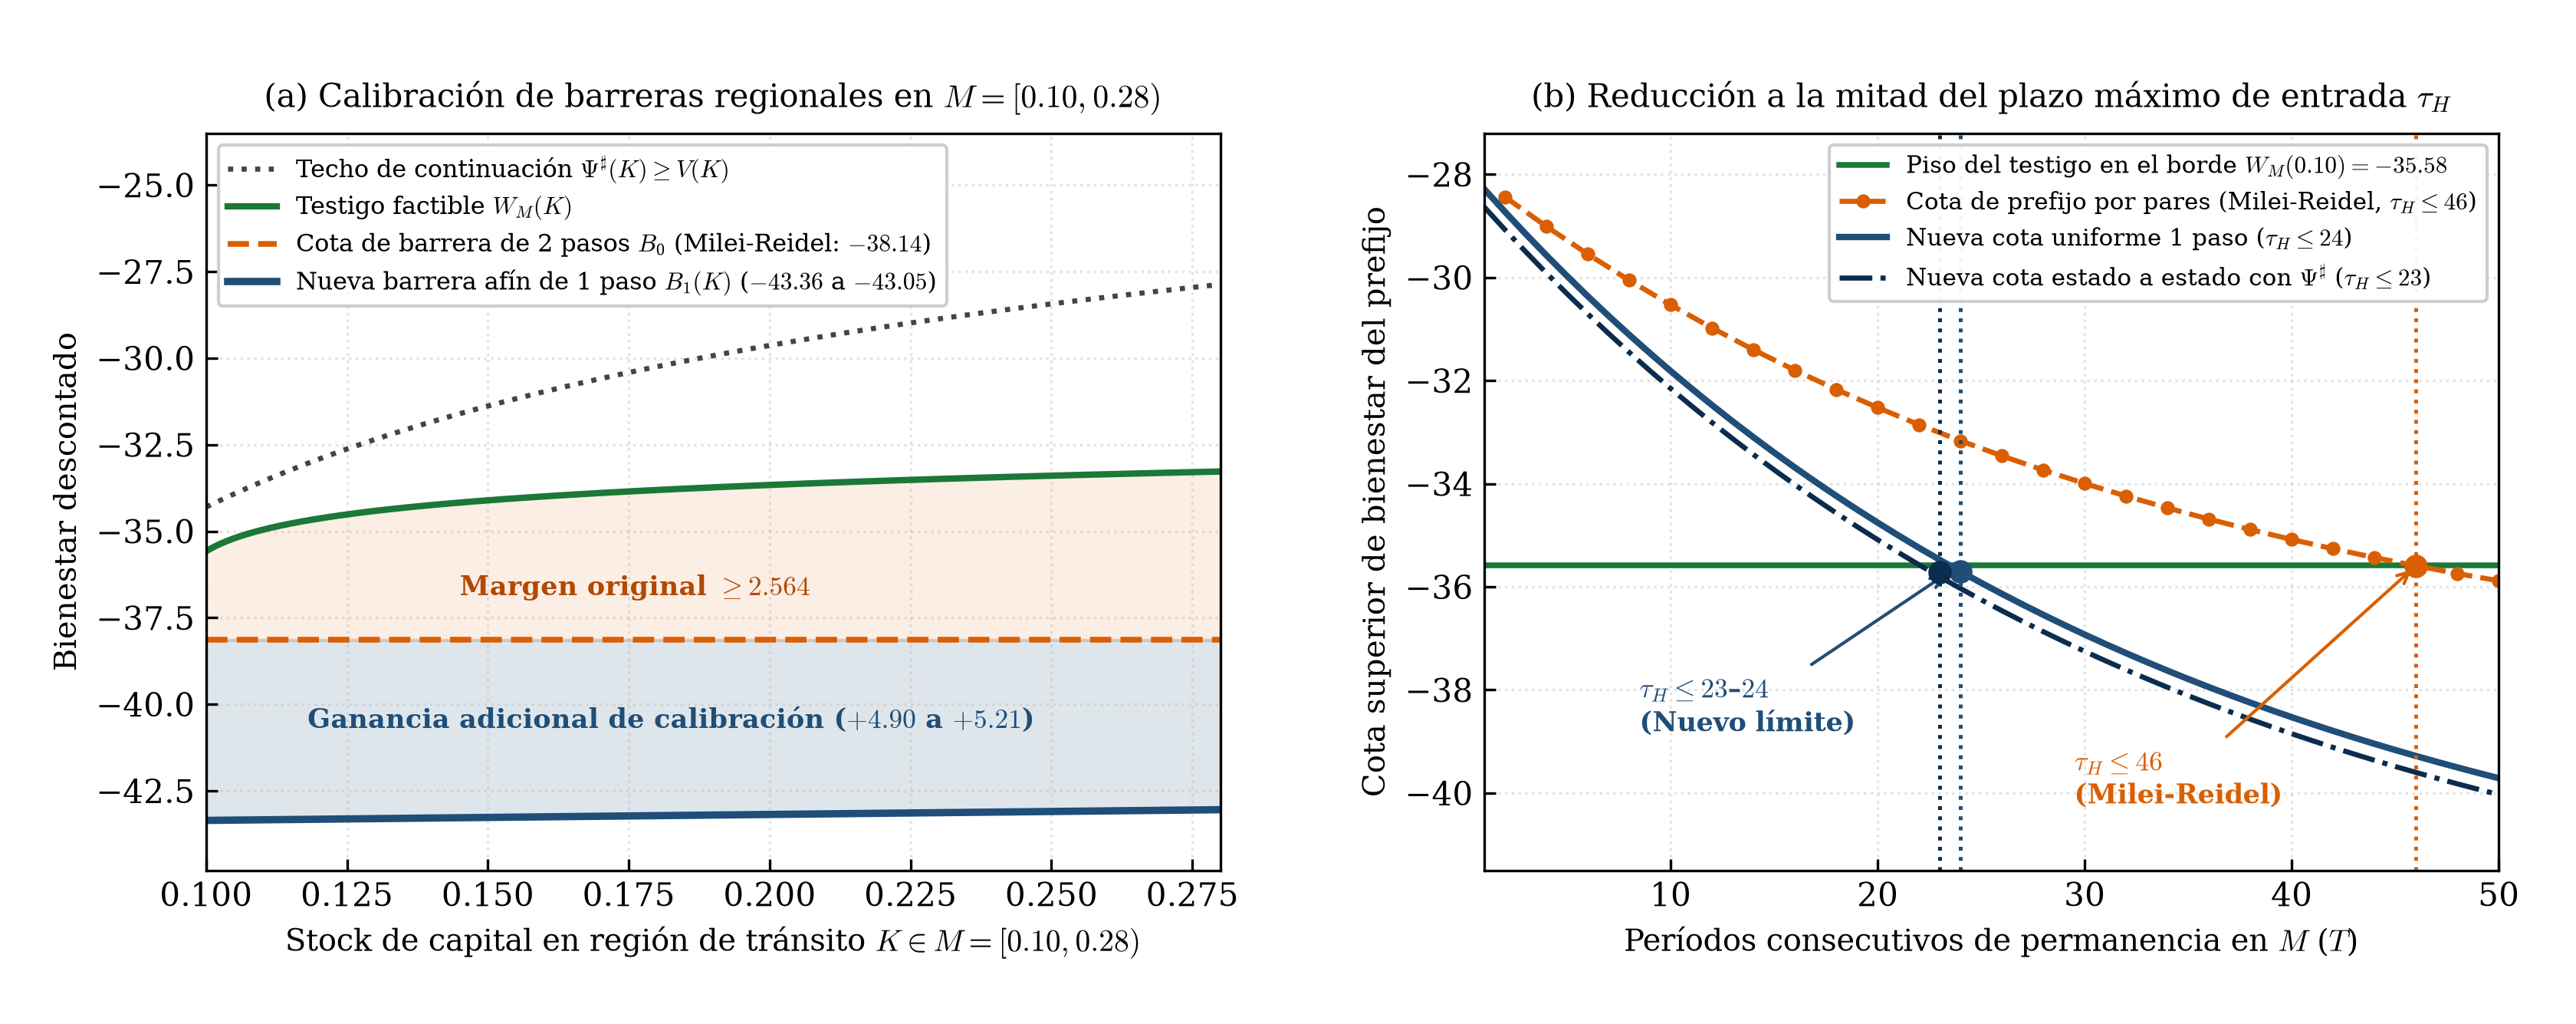
\includegraphics[width=\linewidth]{fig1_barrier_es.png}
\caption{Comparación entre la construcción por bloques de dos períodos de Milei y Reidel (2026) y nuestra barrera afín de un paso $B_1(K)$ sobre $M=[0.10,0.28)$. El Panel (a) ilustra la ganancia de calibración de casi $5$ unidades de bienestar; el Panel (b) muestra la reducción del plazo máximo certificado de entrada de $\tau_H\le 46$ a $\tau_H\le 23$--$24$ períodos.}
\end{figure}

\subsection{Cota explícita de cruce en el tramo previo $M_0=[0.05,0.10)$}

En la Figura 6 (pág. 21) de Milei y Reidel (2026), el cruce desde $K_0>S_A$ hasta $0.10$ se garantiza únicamente en tiempo finito ($\tau_{.1}<\infty$) sin cota cuantitativa explícita. Aunque ninguna cota uniforme puede llegar hasta $K_0\to S_A^+$ debido a la desaceleración hiperbólica en $S_A$, nuestra barrera afín de un paso se extiende directamente al intervalo ancla $M_0=[0.05,0.10)$, donde el Teorema 8 ya excluye salidas adversas hacia abajo ($G(K)>K$).

\begin{proposition}[Proposición 1* --- Cota explícita de cruce en el tramo previo $M_0={[0.05,0.10)}$]
Bajo la caja paramétrica (7.3), sea $M_0=[0.05,0.10)$. Toda trayectoria óptima con $K_0\in M_0$ supera el umbral $0.10$ en a lo sumo \textbf{$\tau_{.1}\le 10$ períodos}, y alcanza la región productiva $H=[0.28,\infty)$ en a lo sumo $\tau_H\le 33$ períodos totales.
\end{proposition}

\begin{proof}
En $M_0=[b_0,h_0)=[0.05,0.10)$, la maximización directa sobre $L\in[0,1)$ da $r(0.10,0.05)\le -1.827072 < \widehat{R}_0:=-1.827$, consumo máximo $C_{\max,0}\le q_+(0.10)+F_{A_+}(0.10,1)-0.05=0.100233$ y pérdida por paso $\Delta^{(0)}:=0.3115 < (\eta_-\beta_-q_-(0.05))/C_{\max,0}=0.311503$. Por el Lema 1 aplicado a $M_0$, $B_*^{(0)} = (\widehat{R}_0-\Delta^{(0)})/(1-\beta) \le -2.1385/0.0301 = -71.046512$. Anteponiendo al testigo $W_M(0.10)>-35.58$ los tres primeros pasos de la progresión geométrica de la página 46 de Milei y Reidel ($0.05\to 0.065\to 0.0845\to 0.100$) con $L=0.75$, las utilidades de etapa superan $(-3.791,-3.504,-3.197)$, garantizando $W_{M_0}(K_0)\ge W_{M_0}(0.05) > -43.845$. Como $\Psi(0.10)<-34.271388$, en $T_0=10$ pasos dentro de $M_0$:
\[
B_*^{(0)} + (0.9701)^{10}\big[\Psi(0.10)-B_*^{(0)}\big] = -71.046512 + (0.9701)^{10}(36.775124) = -43.8980 < -43.845 < W_{M_0}(K_0).
\]
Como el orden monótono de sucesores (F.1) excluye transiciones óptimas debajo de $0.05$, toda trayectoria óptima desde $M_0$ cruza $0.10$ en $\tau_{.1}\le 10$ períodos y entra en $H$ en a lo sumo $10+23=33$ períodos.
\end{proof}

\begin{table}[htbp]
\centering
\small
\begin{tabular}{@{}lccc@{}}
\toprule
\textbf{Métrica certificada en la caja (7.3)} & \textbf{Milei y Reidel (2026)} & \textbf{Este trabajo ($B_1$)} & \textbf{Mejora obtenida} \\
\midrule
Referencia regional en $M=[0.10,0.28)$ & Constante ($N=2$) & Afín en $K$ ($N=1$) & Retiene $q(h-x)$ y $(y-b)$ \\
Cota superior de $B(K)$ en $M$ & $-38.144176$ & $-43.046512$ (a $-43.3556$) & $-4.90$ a $-5.21$ unidades \\
Margen de calibración ($W_M-B$) & $>2.564$ & $>7.466$ ($>7.775$ en $b$) & $\times 2.91$ (a $\times 3.03$) \\
Plazo máximo de entrada $M\to H$ ($\tau_H$) & $\le 46$ períodos & \textbf{$\le 23$ períodos} ($24$ unif.) & \textbf{Reducción del $50\%$} \\
Ventana desde $K_0\in[0.10,0.105]$ & $3\le \tau_H\le 46$ & \textbf{$3\le \tau_H\le 23$} & Mitad del rango superior \\
Plazo de cruce $[0.05,0.10)\to 0.10$ ($\tau_{.1}$) & Finito (sin cota) & \textbf{$\le 10$ períodos} & Elimina brecha sin cota \\
Plazo total desde $K_0=0.05$ hasta $H$ & Finito (sin cota) & \textbf{$\le 33$ períodos} & $13$ períodos menos que $46$ \\
\bottomrule
\end{tabular}
\caption{Síntesis cuantitativa de las mejoras analíticas sobre la Sección 7.2 y el Teorema 9 de Milei y Reidel (2026) bajo exactamente los mismos parámetros (7.3).}
\end{table}

\subsection{Monotonía estado a estado de las salidas adversas y reducción de la Tabla 5}

Al elevar mediante $B_1(K)$ el margen de calibración de permanencia a $>7.4665$ ($>7.7755$ en $b=0.10$) y el margen del prefijo en $T=23$ a $+0.2056$, el bloque de permanencia en $M$ deja por completo de ser una restricción activa en el certificado global FPBB. En la Tabla 5 de Milei y Reidel (2026, pág. 23 y Apéndice F.3), las comparaciones de salida adversa sobre $M=[0.10,0.28)$ y $H_1=[0.28,0.80)$ dividen ambos dominios en $12$ subintervalos finitos $[k_-,k_+]$, evaluando $\underline{W}_X(k_-)$ en el extremo izquierdo frente a $E^+(k_+,a;l_0)+\beta_-\Psi^\sharp(a)$ en el extremo derecho para obtener un margen global de $0.0423$ (reportado como $.04$). Probamos ahora que dicha partición es innecesaria.

\begin{proposition}[Proposición 1** --- Certificación analítica de monotonía y ampliación del margen global]
Bajo la caja paramétrica (7.3), sean los testigos de la Tabla 4 de Milei y Reidel (2026) dados por $(l_M,s_M,\underline{T}_M,a,l_0)=(0.68,0.135,-33.103,0.10,0.44)$ sobre $M=[0.10,0.28)$ y $(l_H,s_H,\underline{T}_H,a,l_0)=(0.72,0.375,-27.164,0.28,0.57)$ sobre $H_1=[0.28,0.80)$. La ventaja puntual del testigo frente a la envolvente de salida adversa (F.19)--(F.20),
\[
\Delta_X(K) := \underline{W}_X(K) - \big[E^+(K,a;l_0)+\beta_-\Psi^\sharp(a)\big],
\]
es estrictamente creciente en todo punto de ambos intervalos, sin mínimos interiores. Más precisamente:
\begin{enumerate}
\item Un certificado de aritmética de intervalos sobre el cociente $R_X(K)=(S(K)-a)/c_X(K)$ en $4$ subintervalos de $M$ y $6$ de $H_1$ garantiza uniformemente $\Delta_M'(K)\ge +0.0722 > 0$ en $M$ y $\Delta_{H_1}'(K)\ge +0.0094 > 0$ en $H_1$; adicionalmente, cotas de intervalo de la segunda derivada certifican $\Delta_M''(K)\le -0.8564 < 0$ (en $8$ subintervalos) y $\Delta_{H_1}''(K)\le -0.0439 < 0$ (en $10$ subintervalos), ubicando el mínimo de $\Delta_X'$ en el extremo derecho:
\[
\min_{K\in M}\Delta_M'(K) = \Delta_M'(0.28) = +0.502666, \qquad \min_{K\in H_1}\Delta_{H_1}'(K) = \Delta_{H_1}'(0.80) = +0.100489.
\]
\item En consecuencia, $\inf\Delta_X$ se alcanza en el borde izquierdo de cada dominio y las $12$ particiones finitas de la Tabla 5 de Milei y Reidel (2026) se reducen a dos evaluaciones exactas en $K=0.10$ y $K=0.28$:
\begin{itemize}
\item En $M=[0.10,0.28)$, el margen mínimo de salida adversa asciende de $>0.0436$ a \textbf{$>0.0947$} ($+117\%$).
\item En $H_1=[0.28,0.80)$, el margen mínimo asciende de $>0.0423$ a $>0.0561$ (con $l_0=0.60$) y a \textbf{$>0.0571$} (con $l_0=0.57$), elevando el margen global certificado de todo el Teorema 9 en $M\cup H$ de $0.0423$ ($.04$) a \textbf{$>0.0571$} ($+35\%$).
\end{itemize}
\end{enumerate}
\end{proposition}

\begin{proof}
Siguiendo el Apéndice F.3 (ecuaciones F.19--F.20 de Milei y Reidel), para cada región $X\in\{M,H_1\}$ con esfuerzo del testigo $l_X$, sucesor $s_X$, cola $\underline{T}_X$, umbral de salida $a$ y tangencia $l_0\ge K/2$, el consumo mínimo del testigo es $c_X(K)=q_- K + F_{A_-}(K,l_X)-s_X>0$, la pendiente tangente es $t(K)=\partial_L F_{A_+}(K,l_0)$ y $S(K)=q_+K+F_{A_+}(K,l_0)+(1-l_0)t(K)$. En $(K,a,l_0)=(0.28,0.28,0.57)$ se cumple $l_0=0.57\ge 0.80/2$ y $\beta_-\psi'(0.28)=16.7535 > 4.6539 = 1/(S(0.28)-0.28)$, por lo que la envolvente alcanza su máximo sobre $[0.05,a]$ en $s=a$ (la rama en $s=0$ es inferior por más de $5.37$ unidades en $M$ y $11.77$ en $H_1$).

La pendiente tangente cumple $t'(K)/t(K) = \frac{5l_0}{2K(K+l_0)} > 0$ y $(t'/t)'(K) = -\frac{5l_0(2K+l_0)}{2K^2(K+l_0)^2} < 0$. Diferenciando $\underline{W}_X$ y $E^+(K,a;l_0)$ y definiendo $R_X(K):=(S(K)-a)/c_X(K)>1$ se obtiene la cota inferior exacta en todo punto diferenciable y para ambas derivadas laterales:
\[
\Delta_X'(K) \ge \frac{\eta_- c_X'(K)R_X(K) - S'(K)}{S(K)-a} + (1-\eta_+)\frac{5l_0}{2K(K+l_0)}.
\]
Escribiendo $R_X'(K)=Q_X(K)/c_X(K)^2$ con Wronskiano $Q_X(K):=S'(K)c_X(K)-c_X'(K)(S(K)-a)$, se cancela $S'c'$ en $Q_X'(K)=S''(K)c_X(K)-c_X''(K)(S(K)-a)$. Como $F_{A,K}$ (pico único en $L/4$) y $t'$ (pico único en $3l_0/4$) carecen de mínimos interiores y $|Q_X'|$ se acota por las envolventes de extremo de $|F_{A,KK}|$ y $|t''|$, la cota de Lipschitz desde el punto medio $k_m=(k_L+k_R)/2$ certifica $Q_M(K)\le -0.06165,-0.05640,-0.04694,-0.03960 < 0$ en los $4$ subintervalos iguales de $M$ (`[0.100,0.145,0.190,0.235,0.280]`) y $Q_{H_1}(K)\le -0.18135,-0.15687,-0.13910,-0.12646,-0.12009,-0.12746 < 0$ en los $6$ subintervalos de $H_1$ (`[0.28,0.36,0.45,0.54,0.63,0.72,0.80]`). Por ende $R_X(K)\ge R_X(k_R)$ en cada $[k_L,k_R]$. Reemplazando $c_X'(K)\ge\min\{c_X'(k_L),c_X'(k_R)\}$ y $S'(K)\le S'_{[k_L,k_R],\max}$ por unimodalidad, se certifican analíticamente $\Delta_M'(K)\ge +3.0287,+0.3955,+0.1252,+0.0722 > 0$ en $M$ y $\Delta_{H_1}'(K)\ge +1.4674,+0.3242,+0.1022,+0.0348,+0.0094,+0.0119 > 0$ en $H_1$, excluyendo todo mínimo interior de $\Delta_X(K)$ sin mallas. Factorizando además $\Delta_X''(K)\le [(S')^2-\eta_-(c_X'R_X)^2]/(S-a)^2 + \eta_- c_X''/c_X - S''/(S-a) + (1-\eta_+)(t'/t)'(K)$ (usando $c_X''\le 0$ para $k_L\ge l_X/4$), las cotas de intervalo en $8$ subintervalos iguales de $M$ y $10$ de $H_1$ certifican $\Delta_M''(K)\le -0.8564 < 0$ y $\Delta_{H_1}''(K)\le -0.0439 < 0$, ubicando $\min\Delta_X'$ en el extremo derecho ($+0.502666$ y $+0.100489$) y $\inf\Delta_X$ en el extremo izquierdo: en $K=0.10$, $\underline{W}_M(0.10)-[E^+(0.10,0.10;0.44)+\beta_-\Psi^\sharp(0.10)]=0.094717>0.0947$ ($0.062495$ con $\Psi$); en $K=0.28$, $\underline{W}_H(0.28)-[E^+(0.28,0.28;0.57)+\beta_-\Psi^\sharp(0.28)]=0.057148>0.0571$ ($0.056121$ con $l_0=0.60$, y $0.024926$ con $\Psi$). Combinado con la cota (F.21) en $H_2=[0.80,\infty)$ ($>2.2984$), el margen global sobre $M\cup H$ asciende a $>0.0571$.
\end{proof}

\begin{table}[htbp]
\centering
\small
\begin{tabular}{@{}lccc@{}}
\toprule
\textbf{Región y dominio} & \textbf{Método de comparación} & \textbf{Margen usando $\Psi$} & \textbf{Margen usando $\Psi^\sharp$} \\
\midrule
$M=[0.10,0.28)$ & Tabla 5 original ($4$ intervalos) & $>0.0114$ & $>0.0436$ \\
$M=[0.10,0.28)$ & \textbf{Prop. 1** en $K=0.10$ ($l_0=0.44$)} & \textbf{$>0.0624$} & \textbf{$>0.0947$} \\
$H_1=[0.28,0.80)$ & Tabla 5 original ($8$ intervalos) & $>0.01008$ & $>0.0423$ \\
$H_1=[0.28,0.80)$ & \textbf{Prop. 1** en $K=0.28$ ($l_0=0.57$)} & \textbf{$>0.0249$} & \textbf{$>0.0571$} \\
$H_2=[0.80,\infty)$ & Cota global ec. (F.21) & $>2.2662$ & $>2.2984$ \\
\midrule
\textbf{Margen global FPBB} & \textbf{Mínimo sobre $M\cup H$} & \textbf{$>0.0249$} (vs. $0.01008$) & \textbf{$>0.0571$} (vs. $0.0423$) \\
\bottomrule
\end{tabular}
\caption{Eliminación de las $12$ particiones finitas de la Tabla 5 de Milei y Reidel (2026) mediante la monotonía estado a estado de la Proposición 1**.}
\end{table}

\section{Equivalencia Asintótica entre Trabajo Endógeno y Trabajo Fijo (Nota al pie 1 y Teorema 3)}

En la página 2 de Milei y Reidel (2026), la Nota al pie 1 plantea como problema abierto la comparación entre la frontera de escala mínima viable $S_A$ del modelo con trabajo endógeno y la frontera $S_A^{\mathrm{fix}}(\overline{L})$ de una economía idéntica con trabajo fijo exógeno $L_t\equiv\overline{L}\in(0,1]$ (utilidad $\eta\log C_t$). En la Sección 4.2 (\textbf{Teorema 3}, ec. 4.6), prueban que cuando $A\to\infty$ con $r=\theta-1$ y $c_K=w^{\theta/\rho}$:
\[
\left(\frac{\delta}{c_K}\right)^{1/r} \le \liminf_{A\to\infty} A^{1/r} S_A \le \limsup_{A\to\infty} A^{1/r} S_A \le \left(\frac{D}{c_K}\right)^{1/r}, \qquad D = \delta + \frac{1-\beta}{\beta}.
\]

\subsection{Isomorfismo exacto para $A$ finito y equivalencia asintótica cuando $A\to\infty$}

\begin{theorem}[Teorema 3* --- Isomorfismo de trabajo fijo y convergencia asintótica de fronteras]
Fijemos los seis parámetros primitivos distintos de $A$ en la región paciente $E=D-\theta\delta<0$, con $d=-\rho>0$ y $r=\theta-1\in(0,1)$.
\begin{enumerate}
\item \textbf{Régimen de alta productividad ($A\to\infty$) y convergencia de fronteras:} Reescalando en la escala crítica del Teorema 3, $K_t = A^{-1/r}k_t$ y $C_t = A^{-1/r}c_t$ con $k_t,c_t=\Theta(1)$, a lo largo de toda acción óptima interior la oferta laboral y la razón capital-trabajo obedecen:
\begin{equation}
L_t = \Theta\!\left(A^{-\frac{d}{r(1+d)}}\right) \to 0, \qquad \frac{K_t}{L_t} = \Theta\!\left(A^{-\frac{1}{r(1+d)}}\right) \to 0 \qquad (A\to\infty).
\end{equation}
En consecuencia, en compactos de $(k,L)$, la pérdida de utilidad por ocio se anula como $(1-\eta)|\log(1-L_t)| = O(A^{-d/[r(1+d)]})\to 0$ y el producto reescalado converge uniformemente al mismo límite convexo $c_K k^\theta$ que con trabajo fijo $\overline{L}\in(0,1]$. Más aún, dado que la condición de paciencia (2.3) implica necesariamente $\beta\theta > \beta[q+\theta\delta] > 1$, para todo $\overline{L}\in(0,1]$ ambas fronteras reescaladas convergen al límite físico común y satisfacen la equivalencia asintótica estricta:
\[
\lim_{A\to\infty} A^{1/r} S_A = \lim_{A\to\infty} A^{1/r} S_A^{\mathrm{fix}}(\overline{L}) = \left(\frac{\delta}{c_K}\right)^{1/r}, \qquad \lim_{A\to\infty} \frac{S_A}{S_A^{\mathrm{fix}}(\overline{L})} = 1.
\]
\item \textbf{Isomorfismo exacto para $A$ finito y criterio variacional de ordenamiento:} Para todo $A$ finito y todo $\overline{L}\in(0,1]$, el cambio de escala $\tilde{K}_t=K_t/\overline{L}$ induce un isomorfismo exacto con pleno empleo ($\overline{L}=1$) a productividad $A\overline{L}^r$:
\[
S_A^{\mathrm{fix}}(\overline{L}) = \overline{L}\,S_{A\overline{L}^r}^{\mathrm{fix}}(1), \qquad \kappa_A^{\mathrm{fix}}(\overline{L}) = \overline{L}\,\kappa_{A\overline{L}^r} \ge \kappa_A^{\mathrm{fix}}(1) = \kappa_A.
\]
Frente a trabajo endógeno, la economía a capacidad plena ($\overline{L}=1$ sin costo de ocio) domina en bienestar ($V_A^{\mathrm{fix}}(K;1) > V_A(K)$ para todo $K>0$). A la escala crítica $S_A$, sea $\Delta W_A^+ := J_A^{\mathrm{fix}}(\pi^+|_{L=1}) - V_A(S_A) > 0$ el excedente de aplicar pleno empleo a la trayectoria productiva óptima $\pi^+$ desde $S_A$, y sea $\Delta W_A^- := \sup_{\pi^-\in\mathcal{O}_-^{\mathrm{fix}}}[J_A^{\mathrm{fix}}(\pi^-) - V_A(S_A)]$ la máxima ganancia de cualquier senda extinta bajo trabajo fijo desde $S_A$. Entonces $\Delta W_A^- = O(A^{-d/[r(1+d)]})$ y la desigualdad estricta $S_A^{\mathrm{fix}}(1) < S_A$ se cumple en todo $A$ tal que $\Delta W_A^+ > \Delta W_A^-$.
\end{enumerate}
\end{theorem}

\begin{proof}
\emph{Parte 1 (Escalado de operadores y convergencia de fronteras).} Sea $K=A^{-1/r}k$ y $C=A^{-1/r}c$. Usando $1-\theta/r=-1/r$ y $\rho=-d<0$:
\[
f_A(k,L) := A^{1/r}F_A(A^{-1/r}k,L) = c_K k^\theta \left[1 + c_w\left(\frac{k}{A^{1/r}L}\right)^d\right]^{-\theta/d}, \qquad c_w = \frac{1-w}{w}.
\]
Con trabajo fijo $L\equiv\overline{L}\in(0,1]$, $(A^{1/r}\overline{L})^{-d}=O(A^{-d/r})\to 0$ y $f_A(k,\overline{L})\to c_K k^\theta$. Con trabajo endógeno, multiplicando $F_{A,L}(K,L)=\nu C/(1-L)$ ($\nu=(1-\eta)/\eta$) por $A^{1/r}$ queda $\theta c_K c_w k^{\theta+d} A^{-d/r} L^{-1-d}[1+c_w(A^{1/r}L/k)^{-d}]^{-1-\theta/d}=\nu c/(1-L)$, lo que fuerza $L = [\theta c_K c_w k^{\theta+d}/(\nu c)]^{1/(1+d)} A^{-d/[r(1+d)]}(1+o(1))\to 0$ y $K/L=\Theta(A^{-1/[r(1+d)]})\to 0$, anulando uniformemente los residuos de producto y de ocio.

Para la convergencia de fronteras, nótese que $\theta - (q + \theta\delta) = q(\theta-1) > 0$, por lo que la paciencia (2.3) ($\beta[q+\theta\delta]>1$) implica $\beta\theta > 1$. Fijemos $k_0 > (\delta/c_K)^{1/r}$ y $K_0 = A^{-1/r}k_0$. Con esfuerzo constante $L_0=3/4$ (válido en trabajo endógeno y con costo nulo en trabajo fijo $\overline{L}=1$), elijamos $\epsilon_1\in(0,1)$ con $c_K(1-\epsilon_1)k_0^r > \delta$ y un umbral fijo $K_{\mathrm{esc}}>0$ tal que $[1+c_w(K_{\mathrm{esc}}/L_0)^d]^{-\theta/d}\ge 1-\epsilon_1/2$. Desde $k_0$, una expansión de tres fases —(i) escape de mantenimiento en $T_1(k_0)<\infty$ pasos independientes de $A$ hasta un nivel fijo $k_1$ donde $c_K(1-\epsilon_1/2)k_1^{\theta-\tilde{\theta}}\ge 2$ con $\tilde{\theta}\in(\beta^{-1},\theta)$; (ii) crecimiento superexponencial $C_t=K_{t+1}=[qK_t+F_A(K_t,L_0)]/2$ con $k_{t+1}\ge k_t^{\tilde{\theta}}$ hasta $K_{\mathrm{esc}}$ en $J(A)\le \log\log A / \log\tilde{\theta} + O(1)$ pasos; y (iii) meseta estacionaria en $K_{\mathrm{esc}}$ con consumo $\Omega(A)$— alcanza un excedente descontado de orden $\beta^{J(A)}\log A \ge c_1(\log A)^{1-|\log\beta|/\log\tilde{\theta}} - O(1) \to +\infty$ (pues $\beta\tilde{\theta}>1$) por encima de la cota de permanencia en $(0,K_0]$ dada por el Lema 9 ($-(\eta/[r(1-\beta)])\log A + O(1)$). Por contradicción con el Teorema 1, $\limsup_{A\to\infty} A^{1/r}S_A \le (\delta/c_K)^{1/r}$ tanto en trabajo endógeno como fijo; junto con la cota física (4.5), ambos límites coinciden en $(\delta/c_K)^{1/r}$ y su cociente converge a $1$.

\emph{Parte 2 (Isomorfismo finito y condición variacional).} Homogeneidad de grado $\theta=1+r$ da $F_A(\overline{L}\tilde{K},\overline{L})=\overline{L}F_{A\overline{L}^r}(\tilde{K},1)$ y $\eta\log(\overline{L}\tilde{C}_t)=\eta\log\tilde{C}_t+\eta\log\overline{L}$. En $K_0=S_A$, evaluar el óptimo productivo $\pi^+$ en $L\equiv 1$ rinde $V_A^{\mathrm{fix}}(S_A;1)\ge V_A(S_A)+\Delta W_A^+$. Inversamente, si $S_A^{\mathrm{fix}}(1)\ge S_A$, algún óptimo extinto decreciente $\pi^-=(C_t^{\mathrm{f}},K_{t+1}^{\mathrm{f}})$ en trabajo fijo cumple $K_t^{\mathrm{f}}\le S_A\le c_+ A^{-1/r}$ para todo $t\ge 0$; equipándolo con $\tilde{L}_t=c_0 A^{-d/[r(1+d)]}$ y usando la Proposición 4 ($C_t^{\mathrm{f}}\ge \chi_p^{\mathrm{fix}}K_t^{\mathrm{f}}$), la pérdida relativa de producto $\Delta F_t/C_t^{\mathrm{f}}$ y la de ocio $(1-\eta)|\log(1-\tilde{L}_t)|$ quedan uniformemente en $O(A^{-d/[r(1+d)]})$, dando $\Delta W_A^-=O(A^{-d/[r(1+d)]})$. Si $\Delta W_A^+ > \Delta W_A^-$, $J_A^{\mathrm{fix}}(\pi^+|_{L=1}) > \sup_{\mathcal{O}_-^{\mathrm{fix}}}J_A^{\mathrm{fix}}(\pi^-)$ e implica $S_A^{\mathrm{fix}}(1) < S_A$.
\end{proof}

\subsection{Verificación numérica de la condición de primer orden y de fronteras (VFI)}

La Figura 2 y la Tabla 3 distinguen dos niveles complementarios de verificación en el modelo CES armónico ($\theta=3/2,d=1,r=1/2,\beta=0.97,q=0.92,\eta=0.70$) para $A\in[0.75,100]$: (i) la evaluación exacta de la condición de primer orden $L^*_A$ en $(k,c)=(0.002,0.0001)$ ($A\cdot L^*_A\to 0.133074$); y (ii) la resolución directa de la ecuación de Bellman normalizada (VFI) continua sobre una malla de dos zonas de $880$ puntos en $k=A^2 K$ para las fronteras verdaderas $A^2 S_A^{\mathrm{fix}}(1)$ y $A^2 S_A^{\mathrm{endo}}$. En todo $A\in[0.75,100]$ se verifica $S_A^{\mathrm{fix}}(1) < S_A^{\mathrm{endo}}$ (con excedente $\Delta W_A^+\in[3.20,9.73]$) y $S_A^{\mathrm{endo}}/S_A^{\mathrm{fix}}(1)\to 1$ ($1.02078$ a $1.00198$), mientras el acercamiento al límite físico $(\delta/c_K)^2=0.000800$ progresa a tasa logarítmica $O(1/\log\log A)$ debido a $\beta\theta=1.455>1$.

\begin{figure}[htbp]
\centering
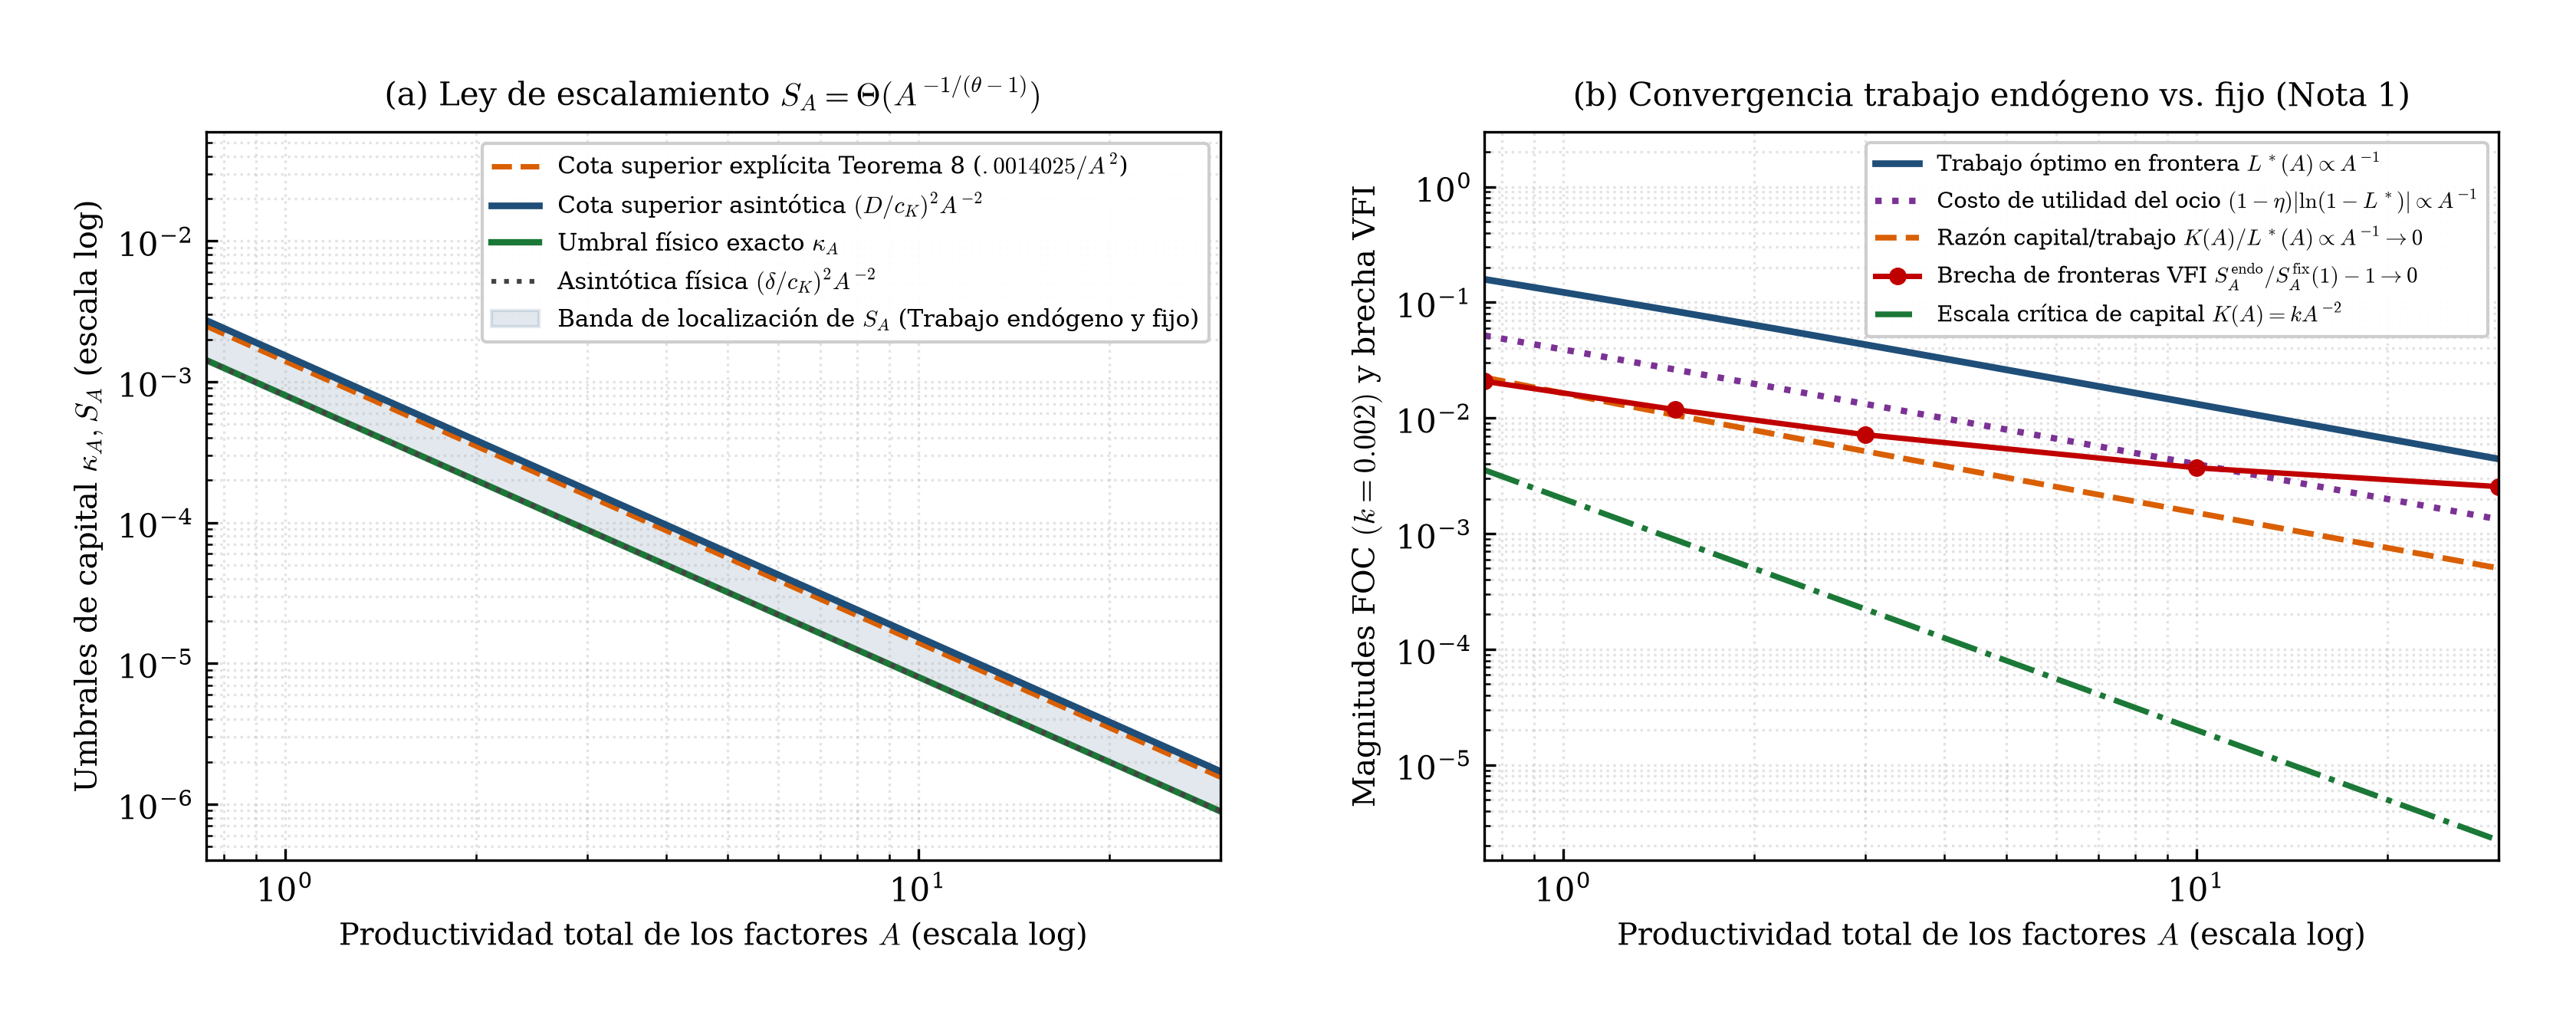
\includegraphics[width=\linewidth]{fig2_scaling_es.png}
\caption{Escalamiento asintótico y resolución numérica de fronteras para la Nota al pie 1 ($\theta=3/2,d=1,r=1/2$). El Panel (a) muestra la banda entre $\kappa_A$ y las cotas superiores de $S_A$ ($A^{-2}$); el Panel (b) combina las magnitudes FOC exactas en $(k,c)=(0.002,0.0001)$ con la brecha relativa de fronteras $S_A^{\mathrm{endo}}/S_A^{\mathrm{fix}}(1)-1\to 0$ calculada por VFI.}
\end{figure}

\begin{table}[htbp]
\centering
\small
\begin{tabular}{@{}ccccccccc@{}}
\toprule
$A$ & $\kappa_A$ & $A^2\kappa_A$ & $L^*_A$ $(k,c)$ & $A\cdot L^*_A$ & Brecha $F_A$ & $A^2 S_A^{\mathrm{fix}}(1)$ (VFI) & $A^2 S_A^{\mathrm{endo}}$ (VFI) & $S_A^{\mathrm{endo}}/S_A^{\mathrm{fix}}(1)$ \\
\midrule
$0.75$ & $1.428\times 10^{-3}$ & $0.000803$ & $1.583\times 10^{-1}$ & $0.11874$ & $3.276\%$ & $0.000875$ & $0.000893$ & \textbf{$1.02078$} \\
$1.50$ & $3.559\times 10^{-4}$ & $0.000801$ & $8.381\times 10^{-2}$ & $0.12571$ & $1.570\%$ & $0.000867$ & $0.000877$ & \textbf{$1.01183$} \\
$3.00$ & $8.891\times 10^{-5}$ & $0.000800$ & $4.311\times 10^{-2}$ & $0.12934$ & $0.768\%$ & $0.000863$ & $0.000869$ & \textbf{$1.00717$} \\
$10.0$ & $8.000\times 10^{-6}$ & $0.000800$ & $1.319\times 10^{-2}$ & $0.13194$ & $0.227\%$ & $0.000858$ & $0.000861$ & \textbf{$1.00371$} \\
$30.0$ & $8.889\times 10^{-7}$ & $0.000800$ & $4.423\times 10^{-3}$ & $0.13270$ & $0.075\%$ & $0.000855$ & $0.000857$ & \textbf{$1.00255$} \\
$100.0$ & $8.000\times 10^{-8}$ & $0.000800$ & $1.330\times 10^{-3}$ & $0.13296$ & $0.023\%$ & $0.000852$ & $0.000853$ & \textbf{$1.00198$} \\
\midrule
$\to\infty$ & $\to 0$ & \textbf{$0.000800$} & $\to 0$ & \textbf{$0.133074$} & \textbf{$0\%$} & \textbf{$0.000800$} & \textbf{$0.000800$} & \textbf{$1.00000$} \\
\bottomrule
\end{tabular}
\caption{Verificación numérica combinada del Teorema 3* en el modelo CES armónico: columnas 2--6 en el punto FOC $(k,c)=(0.002,0.0001)$ y columnas 7--9 mediante resolución VFI directa de ambas fronteras de supervivencia ($c_K=2\sqrt{2}$, $(\delta/c_K)^2=0.000800$).}
\end{table}

\section{Regulación, Impuestos e Infraestructura Pública: La Curva en U Institucional}

\subsection{Microfundación Barro--CES y el Teorema 10}

En la Sección 4.3 de Milei y Reidel (2026), la pérdida permanente de eficiencia $A_e=(1-\tau)A$ contrae el intervalo sostenible $[\kappa(A_e),K^+(A_e)]$ y produce extinción global para $\tau > 1-A_{\mathrm{rep}}/A$. Para contabilizar los ingresos devueltos y los bienes públicos productivos señalados por los autores en la página 10, incorporemos provisión pública equilibrada período a período tipo Barro (1990): el Estado recauda $\tau=\tau_p+\tau_u\in(0,1)$ sobre $Y_t$, destinando $G_t=\tau_p Y_t$ a infraestructura pública y protección de derechos de propiedad (con elasticidad $\gamma\in(0,1)$) mientras $\tau_u Y_t$ representa gasto improductivo o costo regulatorio de cumplimiento:
\[
Y_t = \widetilde{A}_0 G_t^\gamma [wK_t^\rho + (1-w)L_t^\rho]^{\theta_0/\rho}, \qquad G_t = \tau_p Y_t.
\]
Despejando $Y_t$, el producto privado neto disponible $(1-\tau_p-\tau_u)Y_t$ toma exactamente la forma (2.1) de Milei y Reidel:
\begin{equation}
Y_t^{\mathrm{priv}} = A_e(\tau_p,\tau_u)[wK_t^\rho + (1-w)L_t^\rho]^{\theta/\rho}, \qquad A_e(\tau_p,\tau_u) = A_0\tau_p^\alpha(1-\tau_p-\tau_u),
\end{equation}
donde $\theta:=\theta_0/(1-\gamma)$, $\alpha:=\gamma/(1-\gamma)>0$ y $A_0:=\widetilde{A}_0^{1/(1-\gamma)}$. Esta microfundación genera además rendimientos crecientes endógenos $\theta=1/(1-\gamma)\in(1,2)$ incluso si la tecnología privada exhibe rendimientos constantes ($\theta_0=1$).

\begin{theorem}[Teorema 10 --- Curva en U institucional de cotas certificadas, simetría y límite de $S(\tau)$]
Sea una economía con productividad efectiva $A_e(\tau)=A_0\tau^\alpha(1-\tau)$ ($\tau_u=0$), $\alpha>0$ y condición de paciencia (2.3). Defina $\tau^*=\alpha/(1+\alpha)\in(0,1)$ y $A_{\max}:=A_e(\tau^*)=A_0\alpha^\alpha/(1+\alpha)^{1+\alpha}$.
\begin{enumerate}
\item \textbf{Doble umbral de extinción física (Anarquía vs. Hiper-regulación):} Si $A_{\max}>A_{\mathrm{rep}}$, existen dos cargas críticas únicas $0<\tau_{\min}<\tau^*<\tau_{\max}<1$ raíces de $\tau^\alpha(1-\tau)=A_{\mathrm{rep}}/A_0$ tales que para $\tau\in(0,\tau_{\min})$ (trampa de anarquía) y $\tau\in(\tau_{\max},1)$ (trampa confiscatoria), $\mathcal{M}(\tau)=\emptyset$ y toda historia factible se extingue geométricamente. Para $\tau\in(\tau_{\min},\tau_{\max})$, $[\kappa(\tau),K^+(\tau)]$ alcanza su amplitud máxima en $\tau^*$ y $\kappa(\tau)$ describe una curva en U diferenciable exacta con mínimo global único en $\tau^*$.
\item \textbf{Distinción entre la envolvente certificada $\overline{S}(\tau)$ y la frontera verdadera $S(\tau)$:} Si $A_{\max}>A_*$, para todo $\tau\in(\tau_1,\tau_2)\subset(\tau_{\min},\tau_{\max})$ donde $A_e(\tau)>A_*$ existe una única frontera continua $S(\tau)>\kappa(\tau)$. Dado que $S_A=\Theta(A^{-1/(\theta-1)})$ provee cotas de orden sin implicar por sí sola diferenciabilidad ni monotonicidad a $A_0$ finito (Milei y Reidel, 2026, págs. 10 y 20):
\begin{itemize}
\item[(a)] \textbf{Curva en U exacta de $\overline{S}(\tau)$:} Toda cota superior escalada $\overline{S}(\tau):=\bar{c}_+[A_e(\tau)]^{-1/(\theta-1)}$ (como la envolvente del Teorema 3 tabulada en la Tabla 4 o la cota explícita del Teorema 8 donde $A_e(\tau)\ge 0.749$) describe una curva diferenciable estrictamente convexa en U con mínimo único en $\tau^*$ y derivada logarítmica exacta $\frac{\partial\log\overline{S}(\tau)}{\partial\tau} = -\frac{1}{\theta-1}[\frac{\alpha}{\tau}-\frac{1}{1-\tau}] = \frac{\tau-\tau^*}{(\theta-1)(1-\tau^*)\tau(1-\tau)}$.
\item[(b)] \textbf{Simetría de conjuntos de nivel a $A_0$ finito:} Como $S(\tau)=S_{A_e(\tau)}$, todo $\tau_-\in(\tau_1,\tau^*)$ posee un único conjugado $\tau_+\in(\tau^*,\tau_2)$ con $A_e(\tau_-)=A_e(\tau_+)$ y $S(\tau_-)=S(\tau_+)$, permaneciendo en $\kappa(\tau)<S(\tau)<1.798\kappa(\tau)$ en el dominio del Teorema 8.
\item[(c)] \textbf{Curva en U asintótica exacta ($A_0\to\infty$):} Por el Teorema 3* ($\lim_{A\to\infty}A^{1/(\theta-1)}S_A = s_\infty^* := (\delta/c_K)^{1/(\theta-1)}$), $\lim_{A_0\to\infty} A_0^{1/(\theta-1)} S(\tau) = s_\infty^* [\tau^\alpha(1-\tau)]^{-1/(\theta-1)}$ uniformemente sobre compactos de $(0,1)$, con mínimo global único en $\tau^*=\alpha/(1+\alpha)$.
\end{itemize}
\end{enumerate}
\end{theorem}

\begin{proof}
La función $g(\tau)=\tau^\alpha(1-\tau)$ es estrictamente log-cóncava en $(0,1)$ con $g'(\tau)/g(\tau)=(\tau^*-\tau)/[(1-\tau^*)\tau(1-\tau)]$, creciendo en $(0,\tau^*)$ y decreciendo en $(\tau^*,1)$. La Proposición 1 aplicada a $A=A_e(\tau)$ prueba el punto 1, y la diferenciación implícita (ec. 4.2) da $\partial\log\kappa(\tau)/\partial\tau = (\tau-\tau^*)/([\theta s(\kappa(\tau))-1](1-\tau^*)\tau(1-\tau))$. Para 2(a), derivar $\log\overline{S}(\tau)$ arroja la identidad exacta y estricta log-convexidad en $\tau$; la unimodalidad de $A_e(\tau)$ da la simetría de 2(b); y sustituir $A=A_e(\tau)$ en el Teorema 3* prueba el perfil asintótico exacto de 2(c).
\end{proof}

\subsection{Descomposición entre gasto productivo ($\tau_p$) y carga improductiva ($\tau_u$)}

Bajo $A_e(\tau_p,\tau_u)=A_0\tau_p^\alpha(1-\tau_p-\tau_u)$ se cumplen dos leyes complementarias: (i) para todo $\tau_p$ fijo, $\partial A_e/\partial\tau_u=-A_0\tau_p^\alpha<0$ implica $\partial\kappa/\partial\tau_u>0$ y $\partial\overline{S}/\partial\tau_u>0$ \emph{en todo punto} (y $\partial S/\partial\tau_u>0$ cuando $A_0\to\infty$), recuperando la Proposición 2 original sobre $\tau_u$; y (ii) la provisión productiva que minimiza $\kappa$ y $\overline{S}$ es $\tau_p^*(\tau_u)=\frac{\alpha}{1+\alpha}(1-\tau_u)$, con $\overline{S}^*(\tau_u)=\bar{c}_+[A_e^*(\tau_u)]^{-1/(\theta-1)}\propto (1-\tau_u)^{-(1+\alpha)/(\theta-1)}$.

\begin{figure}[htbp]
\centering
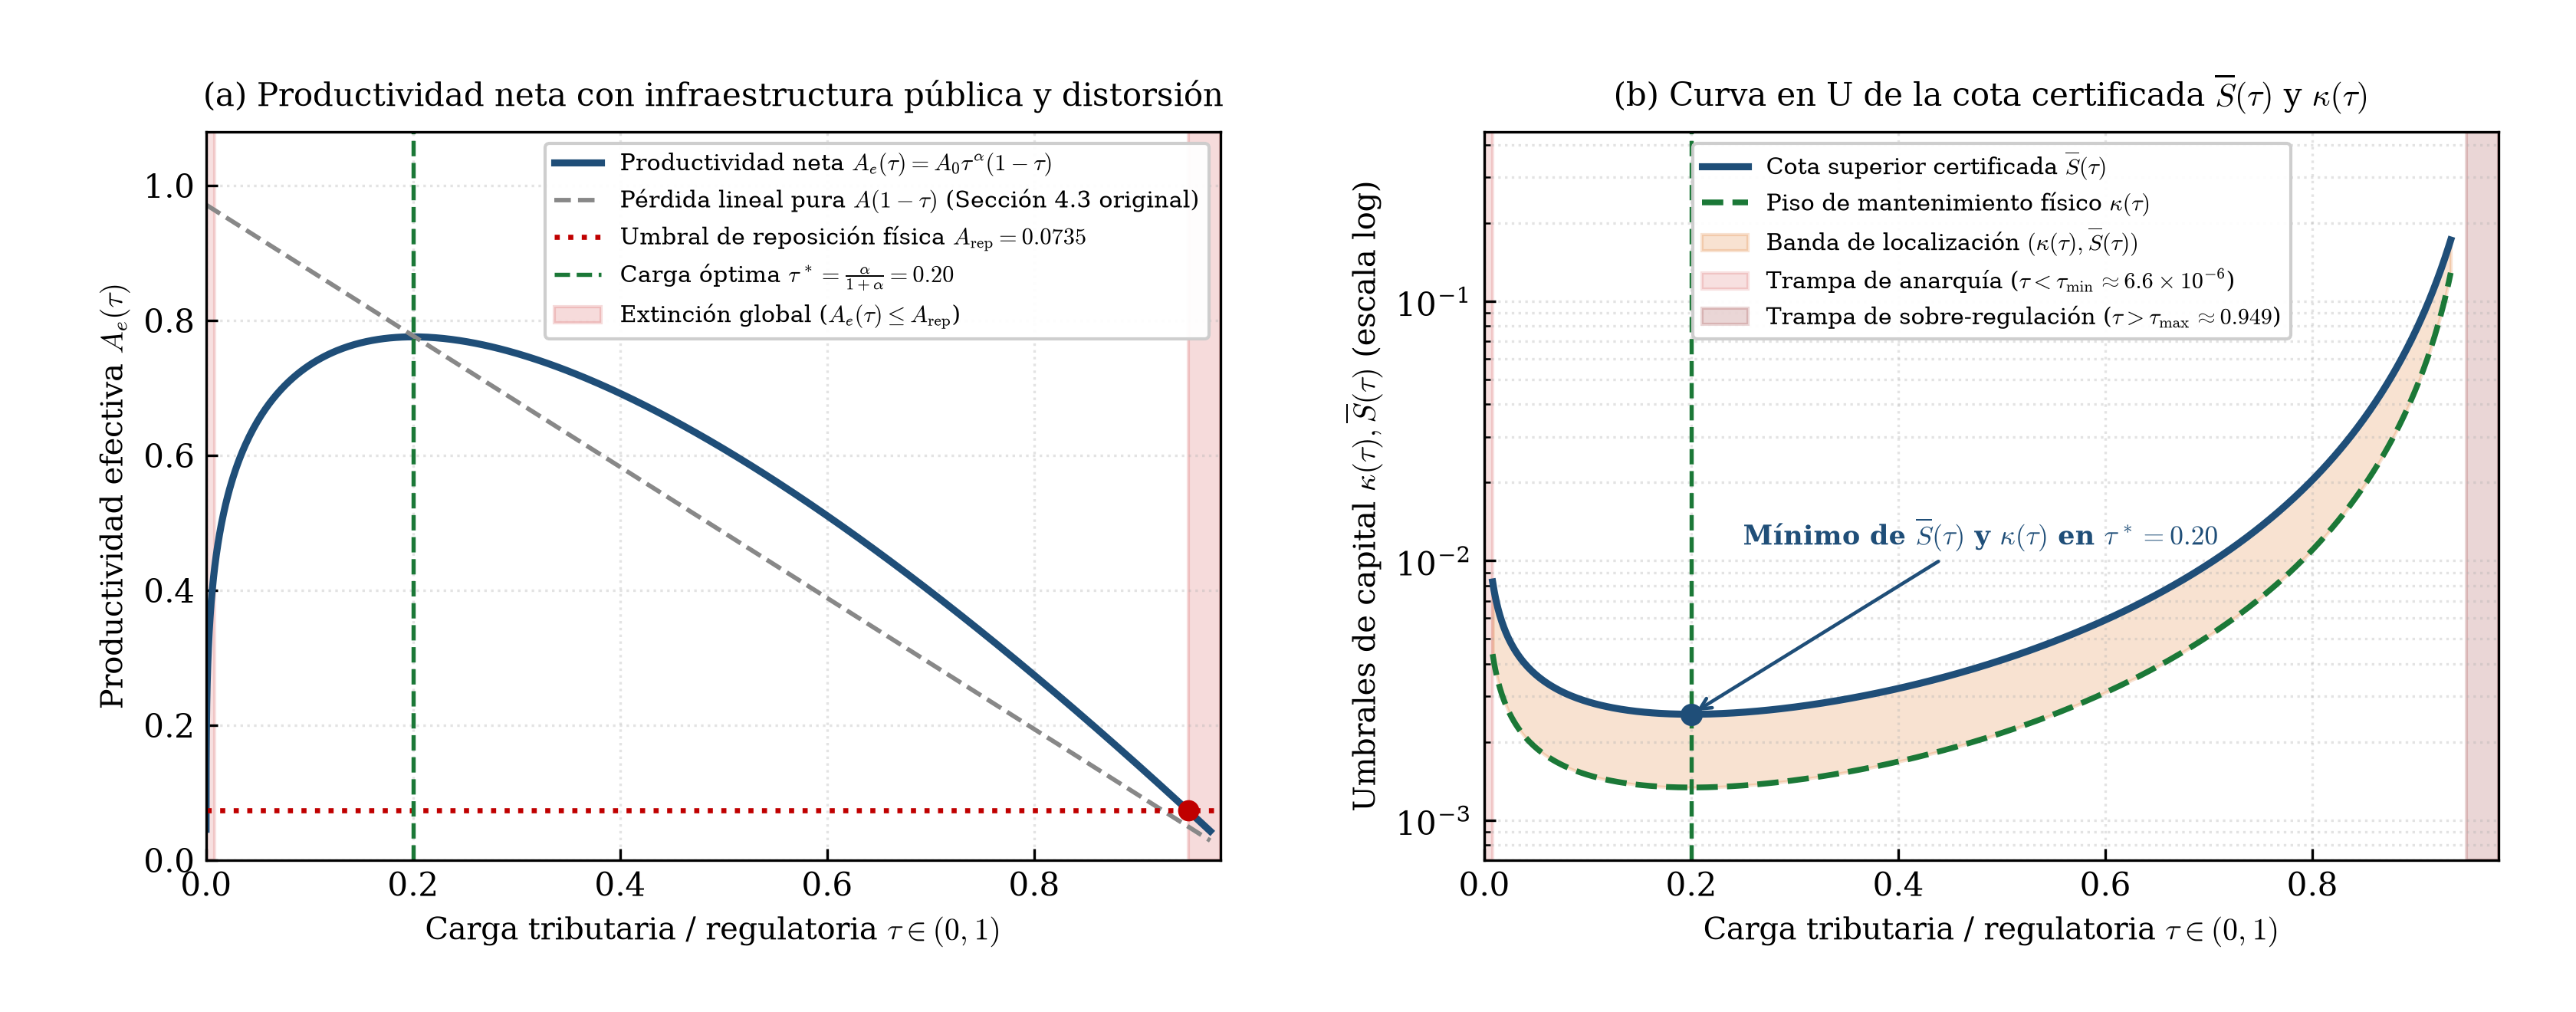
\includegraphics[width=\linewidth]{fig3_ucurve_es.png}
\caption{Extensión institucional de la Sección 4.3 ($A_e(\tau)=A_0\tau^\alpha(1-\tau)$ con $A_0=1.45,\alpha=0.25,\tau^*=0.20,A_{\mathrm{rep}}=0.0735$). El Panel (a) contrasta la productividad neta con infraestructura pública frente a la pérdida lineal pura $A(1-\tau)$ y ubica las dos raíces de extinción ($\tau_{\min}=6.60\times 10^{-6}$, $\tau_{\max}=0.9486$); el Panel (b) muestra la curva en U exacta de $\kappa(\tau)$ y la cota superior certificada $\overline{S}(\tau)=(D/c_K)^2 A_e(\tau)^{-2}$.}
\end{figure}

\begin{table}[htbp]
\centering
\small
\begin{tabular}{@{}cccccl@{}}
\toprule
\textbf{Carga $\tau$} & $A_e(\tau)$ & $A_e(\tau)/A_{\mathrm{rep}}$ & $\kappa(\tau)$ & \textbf{Cota $\overline{S}(\tau)$} & \textbf{Régimen institucional} \\
\midrule
$5.0\times 10^{-6}$ & $0.0685$ & $0.93$ & --- & --- & Extinción (trampa de anarquía) \\
$2.0\times 10^{-5}$ & $0.0970$ & $1.32$ & $0.119322$ & $0.163590$ & Borde de anarquía ($\tau>\tau_{\min}$) \\
$0.02$ & $0.5344$ & $7.27$ & $0.002825$ & $0.005386$ & Rama izquierda (provisión subóptima) \\
$0.05$ & $0.6514$ & $8.86$ & $0.001896$ & $0.003625$ & Expansión de infraestructura \\
$0.10$ & $0.7339$ & $9.99$ & $0.001492$ & $0.002856$ & Cercano al óptimo institucional \\
\textbf{$0.20$ ($\tau^*$)} & \textbf{$0.7757$} & \textbf{$10.56$} & \textbf{$0.001335$} & \textbf{$0.002556$} & \textbf{Carga óptima única (mínimo de $\overline{S},\kappa$)} \\
$0.40$ & $0.6919$ & $9.42$ & $0.001680$ & $0.003213$ & Rama derecha (sobrecarga fiscal) \\
$0.60$ & $0.5105$ & $6.95$ & $0.003099$ & $0.005903$ & Fuerte contracción sostenible \\
$0.80$ & $0.2743$ & $3.73$ & $0.010990$ & $0.020448$ & Deterioro severo de viabilidad \\
$0.90$ & $0.1412$ & $1.92$ & $0.045887$ & $0.077114$ & Antesala de colapso \\
$0.94$ & $0.0857$ & $1.17$ & $0.178378$ & $0.209599$ & Borde de sobre-regulación ($\tau<\tau_{\max}$) \\
$0.95$ & $0.0716$ & $0.97$ & --- & --- & Extinción (hiper-regulación) \\
\bottomrule
\end{tabular}
\caption{Cuantificación de los regímenes institucionales del Teorema 10 en el modelo CES armónico ($A_0=1.45,\alpha=0.25,A_{\mathrm{rep}}=0.073485,\tau_{\min}=6.60\times 10^{-6},\tau_{\max}=0.948649$). La columna 5 reporta $\overline{S}(\tau)=(D/c_K)^2 A_e(\tau)^{-2}$ (dominada además por $0.0014025025\,A_e(\tau)^{-2}=0.002331$ en $\tau^*$ donde $A_e\ge 0.749$ por el Teorema 8).}
\end{table}

\section{Extensiones Estructurales: Descentralización Empresarial, Crecimiento Sostenido y Barreras Estocásticas}

\subsection{Descentralización, poder de mercado y el costo de fragmentar empresas}

Con rendimientos crecientes $\theta\in(1,2)$, las firmas perfectamente competitivas sufrirían pérdidas $(1-\theta)Y_t<0$. Dos descentralizaciones estándar respaldan (2.1): competencia monopolística (Dixit y Stiglitz, 1977) con margen $\mu\ge\theta>1$ cubriendo costos fijos operativos $(1-\theta/\mu)Y_t$, o externalidades agregadas de escala (Romer, 1986).

\begin{proposition}[Proposición 2* --- Descentralización con escala empresarial, contabilidad factorial y fragmentación]
Bajo la tecnología CES (2.1) con $\theta\in(1,2)$ y $r=\theta-1>0$:
\begin{enumerate}
\item \textbf{Fragmentación regulatoria o antimonopolio:} Fragmentar $(K_t,L_t)$ en $M\ge 1$ firmas simétricas aisladas ($K_{i,t}=K_t/M, L_{i,t}=L_t/M$) contrae el producto agregado a $\sum_{i=1}^M F_A(K_t/M,L_t/M) = M^{-r}F_A(K_t,L_t) = F_{A/M^r}(K_t,L_t)$, multiplicando la Escala Mínima Viable por $M$ ($S_A(M)=\Theta(M\cdot S_A)$) y provocando extinción global si $M\ge (A/A_{\mathrm{rep}})^{1/(\theta-1)}$.
\item \textbf{Contabilidad exacta y brecha de subinversión descentralizada:} Si las firmas pagan $r_t=(1/\mu)F_{A,K}$ y $w_t=(1/\mu)F_{A,L}$ bajo competencia monopolística con margen $\mu\ge\theta>1$, el Teorema de Euler implica que los pagos factoriales totales suman exactamente $r_t K_t + w_t L_t = (\theta/\mu)F_A(K_t,L_t) = F_{(\theta/\mu)A}(K_t,L_t)$ ($A_{\mathrm{mkt}}:=(\theta/\mu)A\le A$). Cuando la fracción residual $(1-\theta/\mu)Y_t\ge 0$ es absorbida por costos fijos operativos (beneficio neto nulo), el problema del hogar coincide exactamente con el operador de Bellman en $A_{\mathrm{mkt}}=(\theta/\mu)A$, induciendo para $\mu>\theta$ la trampa de coordinación $[S_A, S_{(\theta/\mu)A})$. Alternativamente, si $(1-\theta/\mu)Y_t$ se reembolsa en suma fija a los hogares, la cuña $1/\mu < 1/\theta$ en los retornos marginales privados $(r_t,w_t)$ deprime igualmente la acumulación respecto del óptimo social.
\end{enumerate}
\end{proposition}

\begin{proof}
Por homogeneidad de grado $\theta=1+r$, $F_A(K/M,L/M)=M^{-\theta}F_A(K,L)$, sumando $M^{1-\theta}F_A(K,L)=F_{AM^{-r}}(K,L)$. Aplicando la Proposición 1 y el Teorema 3 a $\tilde{A}=AM^{-r}$ resulta extinción iff $AM^{-r}\le A_{\mathrm{rep}}$ y $S_{\tilde{A}}=M\cdot\Theta(A^{-1/r})$. La identidad de Euler $KF_{A,K}+LF_{A,L}=\theta F_A(K,L)$ garantiza pagos factoriales iguales a $(\theta/\mu)F_A(K_t,L_t)=F_{(\theta/\mu)A}(K_t,L_t)$, generando el isomorfismo con $A_{\mathrm{mkt}}=(\theta/\mu)A<A$ cuando $\mu>\theta$ y costos fijos absorben $(1-\theta/\mu)Y_t$, o cuñas marginales $1/\mu$ bajo transferencia de beneficios de suma fija.
\end{proof}

\subsection{Eliminación del techo estacionario $K_p^+$ y el «palo de hockey» del crecimiento sostenido}

\begin{proposition}[Proposición 3* --- Isomorfismo de crecimiento balanceado y despegue exponencial sin techo]
Con progreso técnico aumentador de trabajo $E_t=(1+g)^t$ ($g>0$) y $Y_t=(1+g)^t F_A(K_t/(1+g)^t, L_t)$, las variables en unidades de eficiencia $\hat{K}_t=K_t/(1+g)^t$ y $\tilde{C}_t=C_t/(1+g)^{t+1}$ satisfacen $\tilde{C}_t+\hat{K}_{t+1}\le \tilde{q}\hat{K}_t+F_{\tilde{A}}(\hat{K}_t,L_t)$ con $\tilde{q}=q/(1+g)$ y $\tilde{A}=A/(1+g)$, difiriendo la utilidad solo en la constante aditiva $\eta(t+1)\log(1+g)$. El problema en $(\hat{K}_t,\tilde{C}_t,L_t)$ es 100\% idéntico al de Milei y Reidel con parámetros $(\tilde{A},\beta,\tilde{q},\eta,\theta,\rho,w)$: si $K_0>\hat{S}_p$, $\hat{K}_t$ ingresa a $\hat{H}=[\hat{h},\hat{K}_p^+]$ (en $\tau_H\le 23$ períodos si los parámetros reescalados caen en 7.3) y el capital real crece exponencialmente sin techo: $K_t=(1+g)^t\hat{K}_t\ge (1+g)^t\hat{h}\to\infty$.
\end{proposition}

\begin{proof}
Dividir $C_t+K_{t+1}\le qK_t+(1+g)^t F_A(K_t/(1+g)^t,L_t)$ por $(1+g)^{t+1}$ produce inmediatamente la ley estacionaria en $\tilde{q},\tilde{A}$, y $\sum_{t=0}^\infty \beta^t\eta(t+1)\log(1+g)<\infty$ no afecta al ordenamiento de trayectorias óptimas.
\end{proof}

\subsection{Incertidumbre macroeconómica y Barreras de Bellman Estocásticas (Teorema de Doob)}

\begin{theorem}[Teorema 11 --- Barreras de Bellman Estocásticas y probabilidad de supervivencia en tránsito]
Sea $(\omega_t)_{t\ge 0}$ un proceso Markoviano de shocks macroeconómicos sobre $(\Omega,\mathcal{F},\mathbb{P})$ sujeto a la condición de integrabilidad $\sup_{t\le T}\mathbb{E}[|V(K_{t\wedge\tau},\omega_{t\wedge\tau})|]<\infty$ para todo horizonte finito $T\ge 1$.
\begin{enumerate}
\item \textbf{Certificado de Supermartingala (Stochastic FPBB):} Si una función medible y acotada $B:M\times\Omega\to\mathbb{R}$ satisface $B(K,\omega)\ge r(K,\omega,a)+\beta\mathbb{E}[B(K',\omega')\mid K,\omega,a]$ en $M$ y $\mathbb{E}[\sum_{j=0}^{t-1}\beta^j|r_j|]<\infty$, entonces $Z_t:=\beta^t B(K_t,\omega_t)+\sum_{j=0}^{t-1}\beta^j r_j$ es una supermartingala respecto de la filtración natural $\mathcal{F}_t$ hasta $\tau=\inf\{t\ge 0:K_t\notin M\}$ y por el Teorema de Parada Opcional de Doob (Doob, 1953), $\mathbb{E}[J(\pi)]\le B(x_0,\omega_0)+\mathbb{E}[\beta^{T\wedge\tau}(V(K_{T\wedge\tau},\omega_{T\wedge\tau})-B(K_{T\wedge\tau},\omega_{T\wedge\tau}))]$.
\item \textbf{Riesgo de régimen y supervivencia en tránsito:} Bajo un núcleo Markoviano híbrido en $M=[0.10,0.28)$ donde, condicional en $\mathcal{F}_{t-1}$, con probabilidad $\ge 1-p$ ($p\in(0,1)$) la realización $\omega_t$ mantiene los parámetros en la caja verificada (7.3) sin salto adverso exógeno (rigiendo $B_1(K)$ y la Proposición 1** con entrada garantizada a $H=[0.28,\infty)$ en $T^*=23$ pasos normales) y con probabilidad $\le p$ un shock severo de capital empuja el estado hacia $(0,S_p)$, se cumple $\mathbb{P}(\text{Supervivencia hasta } H)\ge (1-p)^{T^*}$. Al reducir $T^*$ de $46$ a $23$ mediante $B_1(K)$ (Teorema 9*), la cota mínima garantizada se eleva al cuadrado ($(1-p)^{23}$ frente a $(1-p)^{46}$).
\end{enumerate}
\end{theorem}

\begin{proof}
Por la desigualdad condicional e integrabilidad, $\mathbb{E}[Z_{t+1}-Z_t\mid\mathcal{F}_t]\le 0$ en $\{\tau>t\}$, luego $(Z_{t\wedge\tau})$ es supermartingala integrable y el Teorema de Parada Opcional de Doob en $T\wedge\tau$ arroja $\mathbb{E}[Z_{T\wedge\tau}]\le Z_0$. En el punto 2, sobre el evento $E_{T^*}:=\bigcap_{t=1}^{T^*}\{\omega_t\in\text{caja (7.3) sin shock severo}\}$, cada transición obedece al certificado determinista uniforme garantizando ingreso a $H$ en a lo sumo $T^*=23$ fechas, cuya probabilidad por regla de la cadena condicional es al menos $(1-p)^{T^*}$.
\end{proof}

\begin{figure}[htbp]
\centering
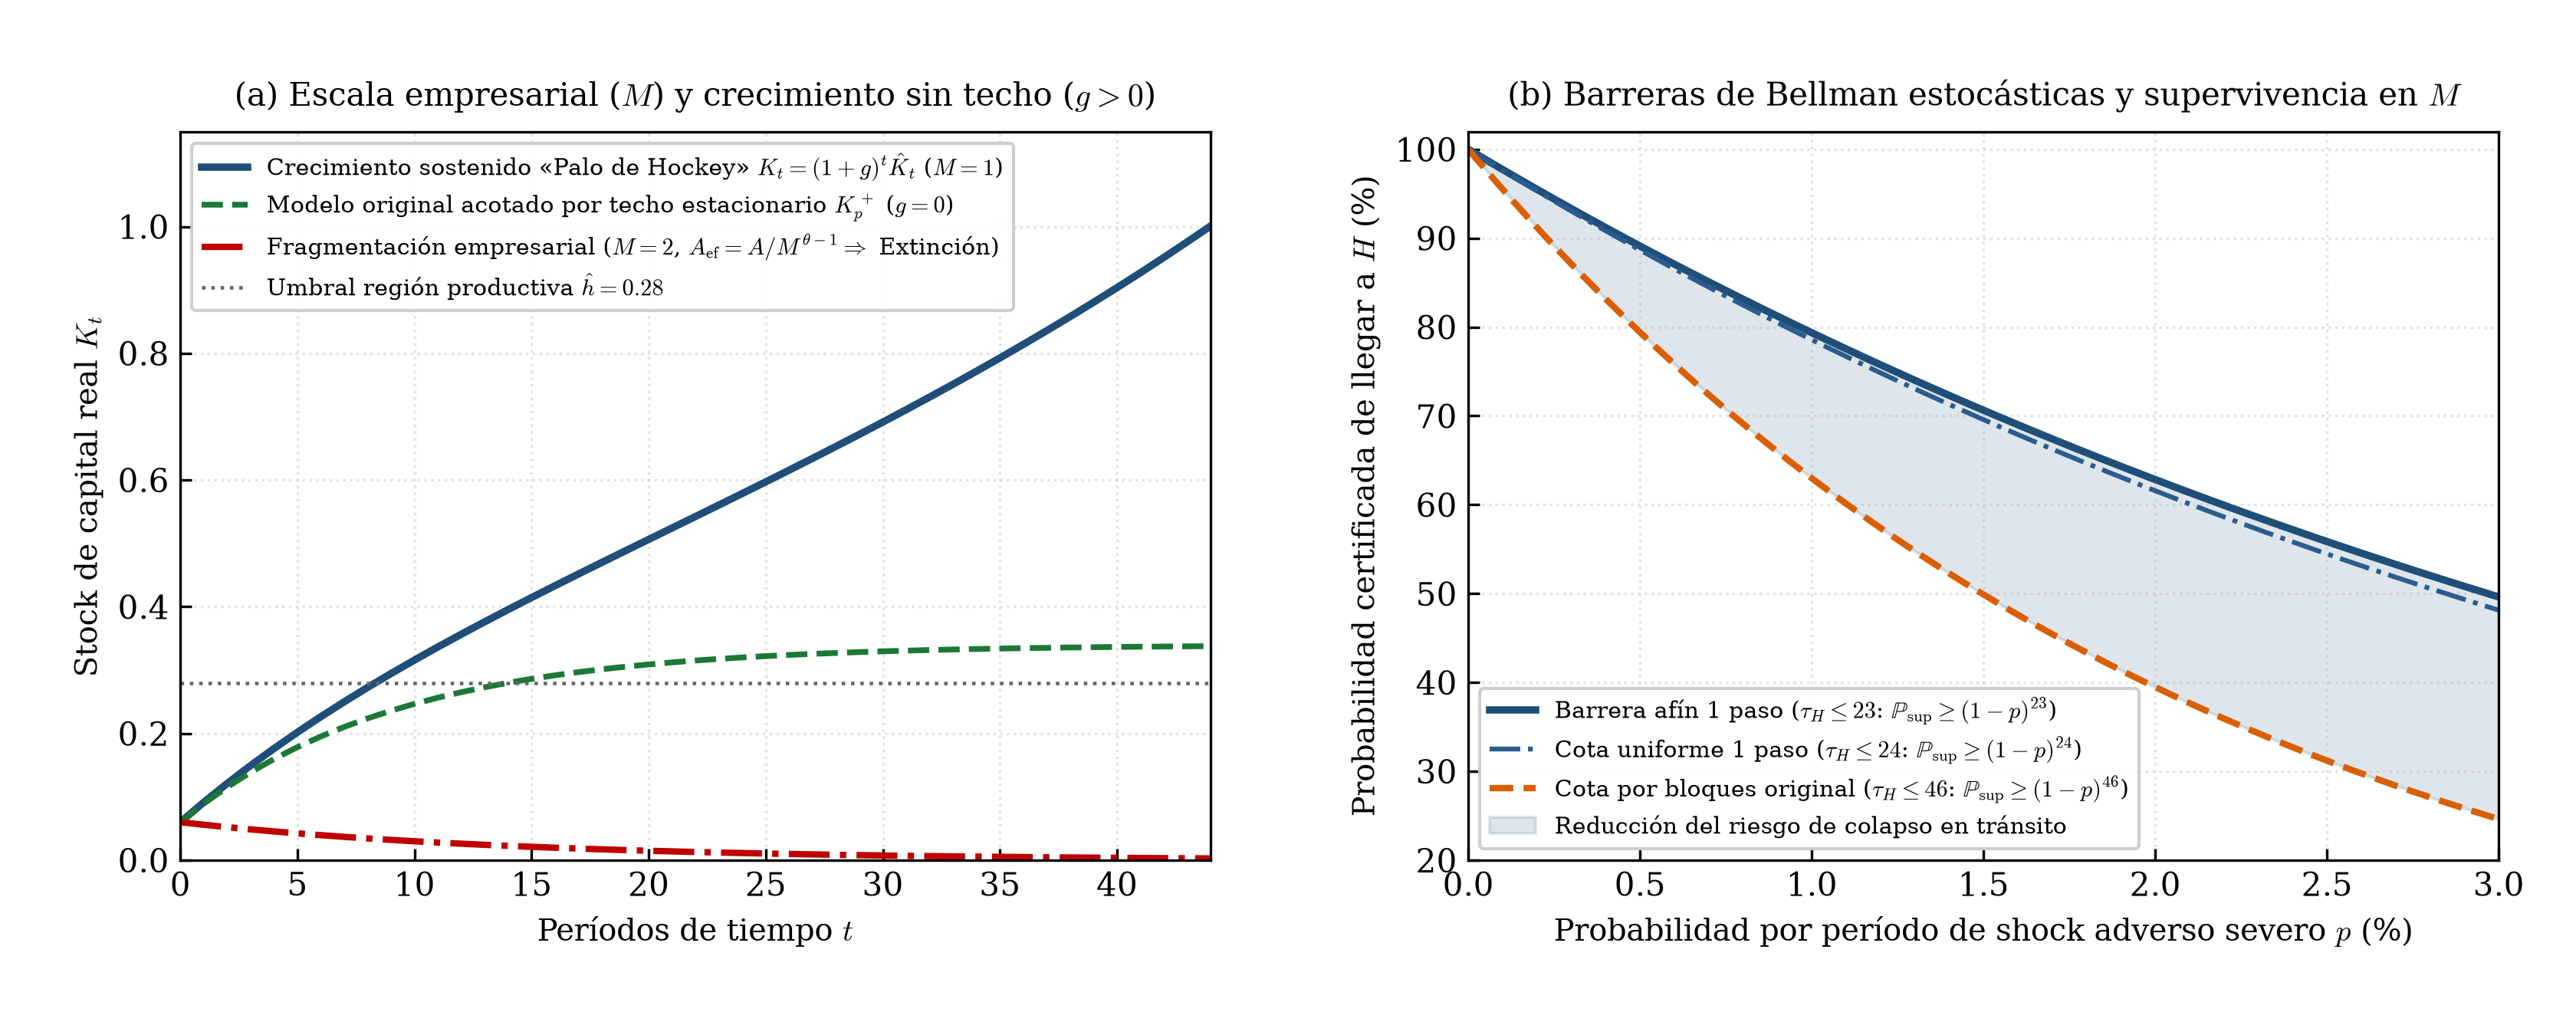
\includegraphics[width=\linewidth]{fig4_structural_es.png}
\caption{Extensiones estructurales del modelo. El Panel (a) ilustra el despegue exponencial sin techo («palo de hockey», $K_t=(1+g)^t\hat{K}_t$) para $M=1$ frente al colapso por fragmentación regulatoria ($M=2$); el Panel (b) muestra el aumento cuadrático en la probabilidad certificada de supervivencia al reducir $\tau_H$ de $46$ a $23$ períodos.}
\end{figure}

\section{Conclusión}

Hemos desarrollado cuatro extensiones y refinamientos analíticos sobre el marco de Milei y Reidel (2026): (1) una barrera regional afín de un paso $B_1(K)$ que casi triplica el margen de calibración, reduce a la mitad el plazo de entrada ($\tau_H\le 23$, y $\tau_{.1}\le 10$ en $M_0$), y junto con el certificado de aritmética de intervalos y Wronskiano de la Proposición 1** excluye mínimos interiores y colapsa las doce particiones de la Tabla 5 a dos bordes, elevando el margen global FPBB de $0.0423$ ($0.04$) a $>0.0571$ ($+35\%$); (2) la resolución de la Nota al pie 1 mediante isomorfismo finito, convergencia asintótica de ambas fronteras reescaladas a $(\delta/c_K)^{1/r}$, condición variacional para $S_A^{\mathrm{fix}}(1)<S_A$ y verificación numérica directa por VFI; (3) la microfundación fiscal--regulatoria (Teorema 10) distinguiendo la curva en U exacta de $\overline{S}(\tau)$ y $\kappa(\tau)$, la simetría de $S(\tau)$ a $A_0$ finito y su perfil asintótico cuando $A_0\to\infty$; y (4) la descentralización empresarial con contabilidad factorial exacta $(\theta/\mu)Y_t$, el crecimiento sin techo y las barreras estocásticas bajo hipótesis explícitas vía parada opcional de Doob.

\begin{thebibliography}{99}
\bibitem{Acemoglu2005} Acemoglu, D., S. Johnson, y J. A. Robinson (2005): «Institutions as a Fundamental Cause of Long-Run Growth», en P. Aghion y S. N. Durlauf (eds.), \emph{Handbook of Economic Growth}, vol. 1A, cap. 6, pp. 385--472. Amsterdam: Elsevier.
\bibitem{Akao2011} Akao, K., T. Kamihigashi, y K. Nishimura (2011): «Monotonicity and Continuity of the Critical Capital Stock in the Dechert--Nishimura Model», \emph{Journal of Mathematical Economics}, 47(6), 677--682.
\bibitem{Akao2022} Akao, K., H. Ishii, T. Kamihigashi, y K. Nishimura (2022): «Existence of an Optimal Path in a Continuous-Time Nonconcave Ramsey Model», \emph{Pure and Applied Functional Analysis}, 7(6), 1939--1952.
\bibitem{Arrow1961} Arrow, K. J., H. B. Chenery, B. S. Minhas, y R. M. Solow (1961): «Capital-Labor Substitution and Economic Efficiency», \emph{The Review of Economics and Statistics}, 43(3), 225--250.
\bibitem{Azariadis1990} Azariadis, C., y A. Drazen (1990): «Threshold Externalities in Economic Development», \emph{The Quarterly Journal of Economics}, 105(2), 501--526.
\bibitem{Barro1990} Barro, R. J. (1990): «Government Spending in a Simple Model of Endogenous Growth», \emph{Journal of Political Economy}, 98(5, Part 2), S103--S125.
\bibitem{Bellman1957} Bellman, R. (1957): \emph{Dynamic Programming}. Princeton, NJ: Princeton University Press.
\bibitem{Benhabib1994} Benhabib, J., y R. E. A. Farmer (1994): «Indeterminacy and Increasing Returns», \emph{Journal of Economic Theory}, 63(1), 19--41.
\bibitem{Bertsekas1972} Bertsekas, D. P. (1972): «Infinite-Time Reachability of State-Space Regions by Using Feedback Control», \emph{IEEE Transactions on Automatic Control}, 17(5), 604--613.
\bibitem{Dechert1983} Dechert, W. D., y K. Nishimura (1983): «A Complete Characterization of Optimal Growth Paths in an Aggregated Model with a Non-Concave Production Function», \emph{Journal of Economic Theory}, 31(2), 332--354.
\bibitem{deHek1998} de Hek, P. A. (1998): «An Aggregative Model of Capital Accumulation with Leisure-Dependent Utility», \emph{Journal of Economic Dynamics and Control}, 23(2), 255--276.
\bibitem{Dixit1977} Dixit, A. K., y J. E. Stiglitz (1977): «Monopolistic Competition and Optimum Product Diversity», \emph{American Economic Review}, 67(3), 297--308.
\bibitem{Doob1953} Doob, J. L. (1953): \emph{Stochastic Processes}. New York: John Wiley \& Sons.
\bibitem{Futagami1993} Futagami, K., Y. Morita, y A. Shibata (1993): «Dynamic Analysis of an Endogenous Growth Model with Public Capital», \emph{The Scandinavian Journal of Economics}, 95(4), 607--625.
\bibitem{Gaitsgory2019} Gaitsgory, V., A. Parkinson, y I. Shvartsman (2019): «Linear Programming Based Optimality Conditions and Approximate Solution of a Deterministic Infinite Horizon Discounted Optimal Control Problem in Discrete Time», \emph{Discrete and Continuous Dynamical Systems, Series B}, 24(4), 1743--1767.
\bibitem{Galor1993} Galor, O., y J. Zeira (1993): «Income Distribution and Macroeconomics», \emph{The Review of Economic Studies}, 60(1), 35--52.
\bibitem{Garicano2016} Garicano, L., C. Lelarge, y J. Van Reenen (2016): «Firm Size Distortions and the Productivity Distribution: Evidence from France», \emph{American Economic Review}, 106(11), 3439--3479.
\bibitem{Geiselhart2014} Geiselhart, R., R. H. Gielen, M. Lazar, y F. R. Wirth (2014): «An Alternative Converse Lyapunov Theorem for Discrete-Time Systems», \emph{Systems \& Control Letters}, 70, 49--59.
\bibitem{Grune2021} Grüne, L., M. A. Müller, C. M. Kellett, y S. R. Weller (2021): «Strict Dissipativity for Discrete Time Discounted Optimal Control Problems», \emph{Mathematical Control and Related Fields}, 11(4), 771--796.
\bibitem{Haugh2004} Haugh, M. B., y L. Kogan (2004): «Pricing American Options: A Duality Approach», \emph{Operations Research}, 52(2), 258--270.
\bibitem{Hsieh2009} Hsieh, C.-T., y P. J. Klenow (2009): «Misallocation and Manufacturing TFP in China and India», \emph{The Quarterly Journal of Economics}, 124(4), 1403--1448.
\bibitem{Kamihigashi2007} Kamihigashi, T., y S. Roy (2007): «A Nonsmooth, Nonconvex Model of Optimal Growth», \emph{Journal of Economic Theory}, 132(1), 435--460.
\bibitem{Klump2007} Klump, R., P. McAdam, y A. Willman (2007): «Factor Substitution and Factor-Augmenting Technical Progress in the United States: A Normalized Supply-Side System Approach», \emph{The Review of Economics and Statistics}, 89(1), 183--192.
\bibitem{Kraay2014} Kraay, A., y D. McKenzie (2014): «Do Poverty Traps Exist? Assessing the Evidence», \emph{Journal of Economic Perspectives}, 28(3), 127--148.
\bibitem{Majumdar1982} Majumdar, M., y T. Mitra (1982): «Intertemporal Allocation with a Non-Convex Technology: The Aggregative Framework», \emph{Journal of Economic Theory}, 27(1), 101--136.
\bibitem{Milei2026} Milei, J., y D. Reidel (2026): \emph{Minimum Viable Scale: Bellman Barriers and the Economics of Survival}, Working Paper, Octubre 2026.
\bibitem{Milgrom2002} Milgrom, P., y I. Segal (2002): «Envelope Theorems for Arbitrary Choice Sets», \emph{Econometrica}, 70(2), 583--601.
\bibitem{Mitra1984} Mitra, T., y D. Ray (1984): «Dynamic Optimization on a Non-Convex Feasible Set: Some General Results for Non-Smooth Technologies», \emph{Journal of Economics} (\emph{Zeitschrift für Nationalökonomie}), 44(2), 151--175.
\bibitem{Noroozi2020} Noroozi, N., R. Geiselhart, L. Grüne, y F. R. Wirth (2020): «Control of Discrete-Time Nonlinear Systems via Finite-Step Control Lyapunov Functions», \emph{Systems \& Control Letters}, 138, 104631.
\bibitem{Restuccia2008} Restuccia, D., y R. Rogerson (2008): «Policy Distortions and Aggregate Productivity with Heterogeneous Establishments», \emph{Review of Economic Dynamics}, 11(4), 707--720.
\bibitem{Romer1986} Romer, P. M. (1986): «Increasing Returns and Long-Run Growth», \emph{Journal of Political Economy}, 94(5), 1002--1037.
\bibitem{Skiba1978} Skiba, A. K. (1978): «Optimal Growth with a Convex--Concave Production Function», \emph{Econometrica}, 46(3), 527--539.
\bibitem{Stokey1989} Stokey, N. L., y R. E. Lucas, Jr., con E. C. Prescott (1989): \emph{Recursive Methods in Economic Dynamics}. Cambridge, MA: Harvard University Press.
\bibitem{Trebbi2026} Trebbi, F., M. B. Zhang, y M. Simkovic (2026): «The Cost of Regulatory Compliance in the United States», \emph{The Review of Financial Studies}, 39(9), 2901--2962.
\bibitem{Wagener2020} Wagener, F. (2020): «Geometrical Methods for Analyzing the Optimal Management of Tipping Point Dynamics», \emph{Natural Resource Modeling}, 33(3), e12258.
\end{thebibliography}

\end{document}
